
\section{Experimental Results on Synthetic Data}\label{sec:synData}
\subsection{Synthetic Scalar and Gradient Data} 
\begin{figure*}[tb]
	\subfloat[]{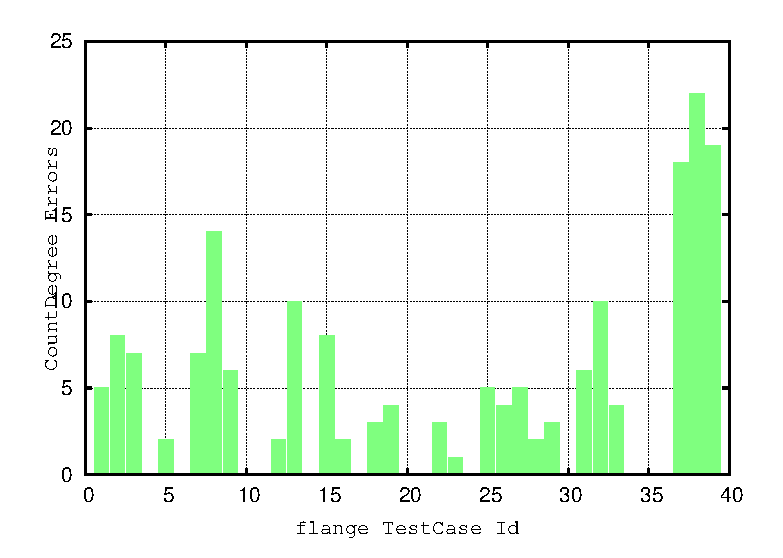
\includegraphics[width=0.33\linewidth]{images/flangeAngle3.eps}\label{fig:flangeAngle3}}
	\subfloat[]{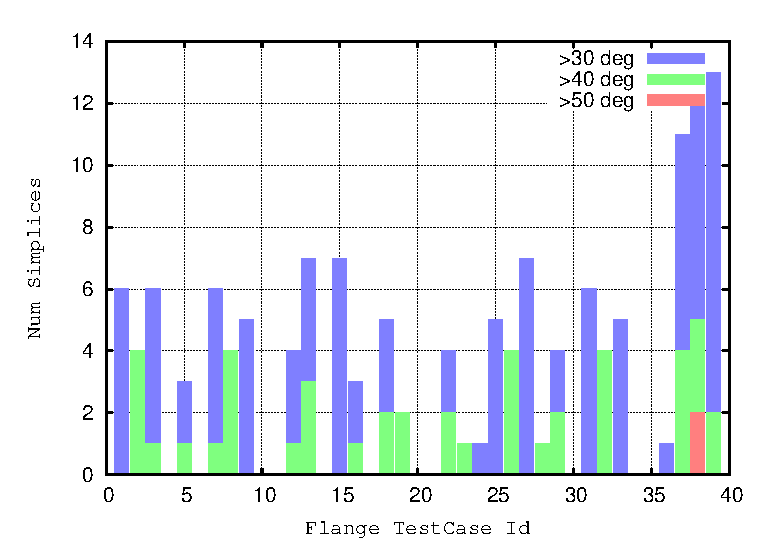
\includegraphics[width=0.33\linewidth]{images/flangeAngle1.eps}\label{fig:flangeAngle1}}
	\subfloat[]{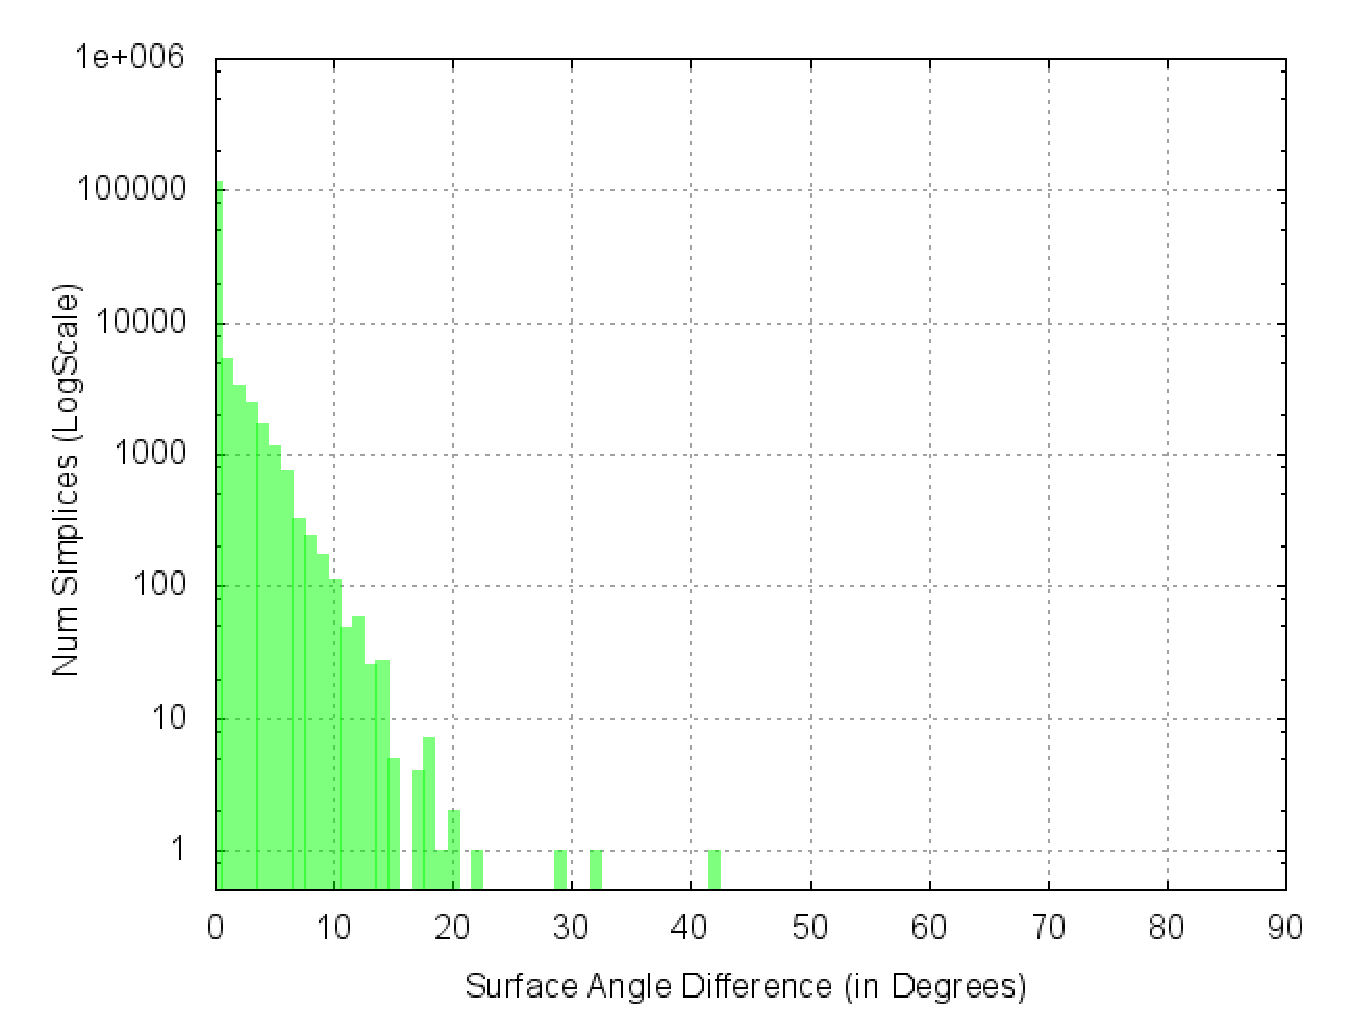
\includegraphics[width=0.33\linewidth]{images/flangeAngle2.eps}\label{fig:flangeAngle2}}
	\caption{SHREC with gradients computed from scalar data using RELIGRAD on 40 datasets. (a) Number of CountDegree errors. (b) Number of simplices with angle difference to ``perfect" mesh above 30, 40 and 50 degrees. (b) Shows the angle distribution of one particular case (16) which has three simplices over 30 degrees and 1 above 40 degrees. Total number of simplices is ~133k.}\label{fig:flangeAngle}
\end{figure*}
\subsection{Isosurface Reconstruction on Synthetic Data}
Figure~\ref{fig:flangeAngle} shows the summary results of running algorithm SHREC on 40 flange datasets. Figure~\protect\subref*{fig:flangeAngle3} shows the number of CountDegree errors in running SHREC with gradients computed from the scalar volume using RELIGRAD.
14 cases ($35\%$) produced no degree errors. The mean error was 4.5. The maximum error was 22.
Figure~\protect\subref*{fig:flangeAngle1} shows the number of simplices with angle difference greater than 30, 40 and 50 degrees, from the original mesh for the 40 test cases. Figure~\protect\subref*{fig:flangeAngle2} shows  the number of simplices versus the angle difference for one particular dataset(16). The particular dataset has no degree errors, it has three simplices with surface angle difference greater than 30 degrees to the original and one simplex above 40 degrees. The mesh itself has approximately 133 thousand simplices. With perfect gradient SHREC produced ``NO" degree errors on the 40 test cases. 
Figure~\ref{fig:flange1} shows the result on a particular dataset. The magnified region shows sharp edges blended with the mesh edges. 
%\begin{figure}[ht]
%	\subfloat[]{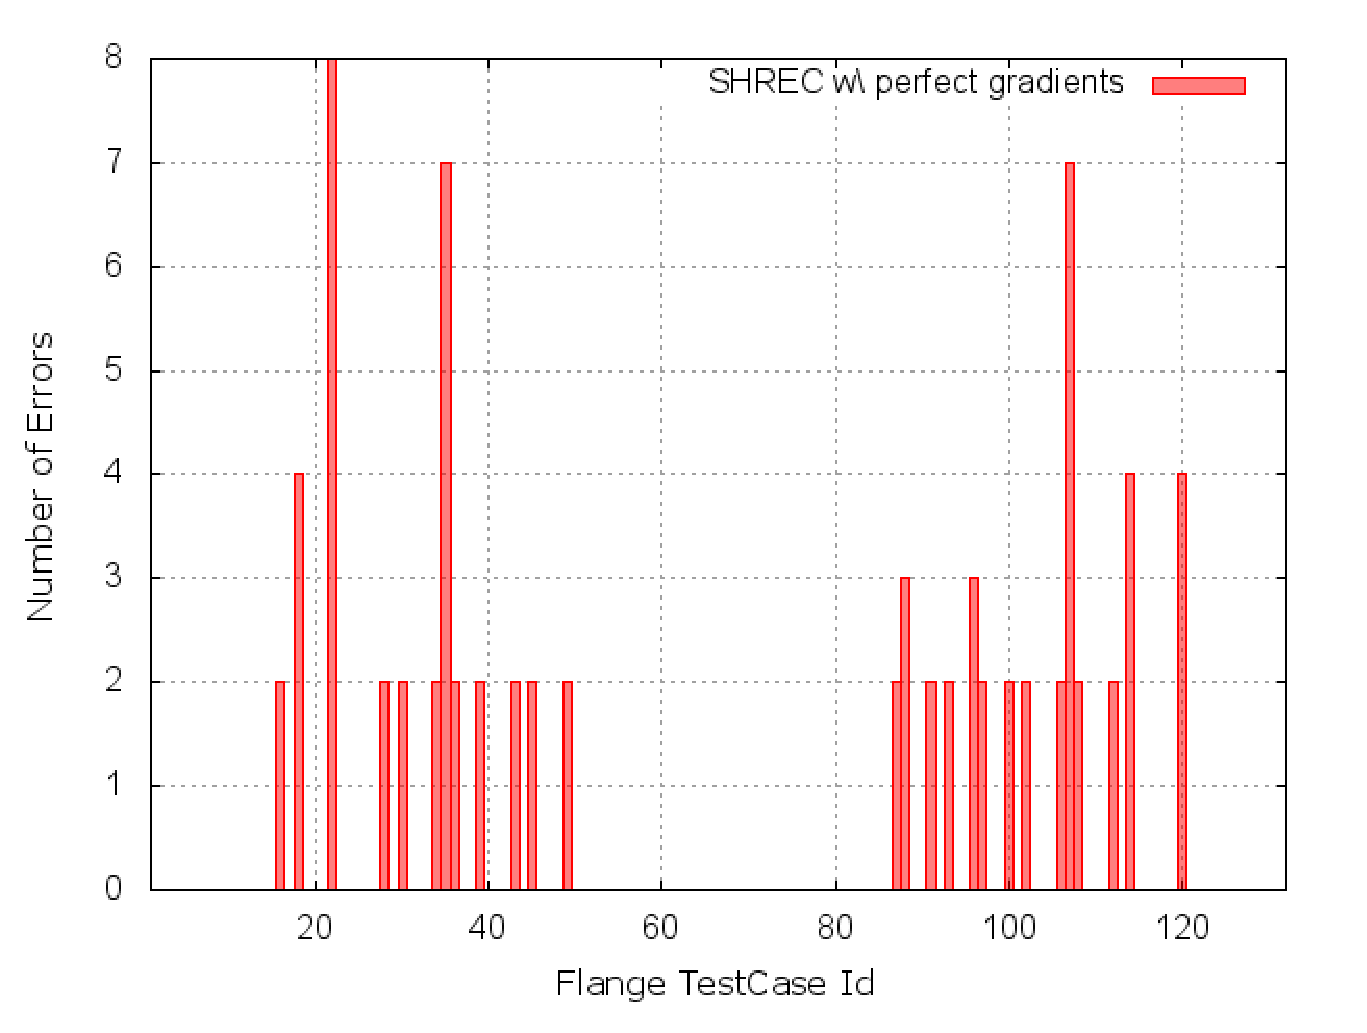
\includegraphics[width=0.5\linewidth]{images/shrecFlange1.eps}\label{fig:shrecFlange:1}}
%	\subfloat[]{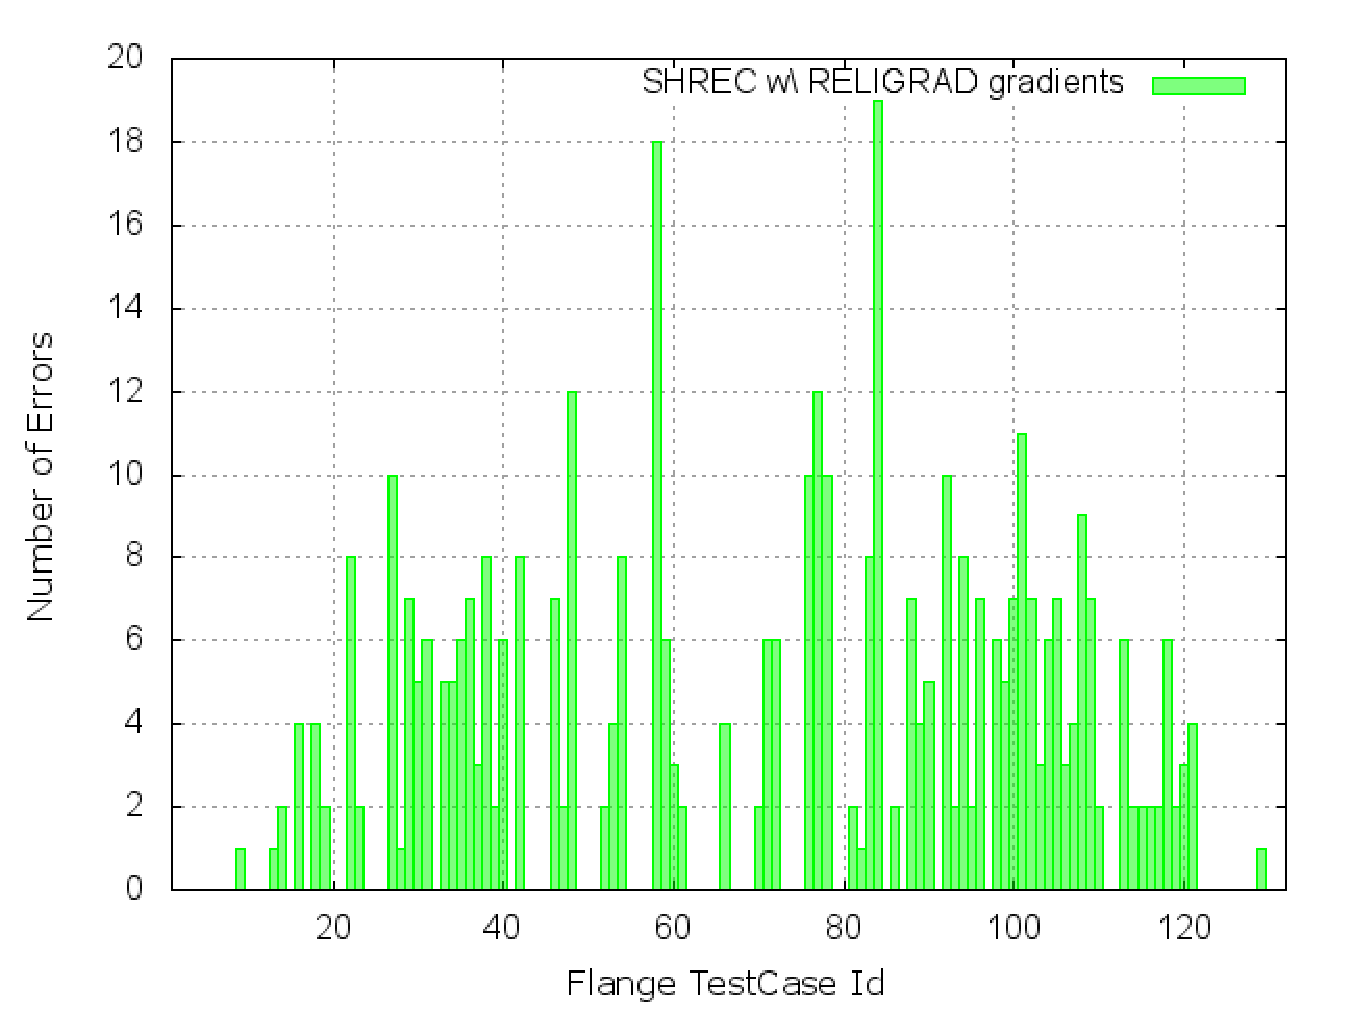
\includegraphics[width=0.5\linewidth]{images/shrecFlange2.eps}\label{fig:shrecFlange:2}}
%	\caption{Results of Shrec on 132 Flange data sets. (a) Shrec with perfect gradients. (b) Shrec with Religrad gradients.}
%	\label{fig:shrecFlange}
%\end{figure}
\begin{figure}[tb]
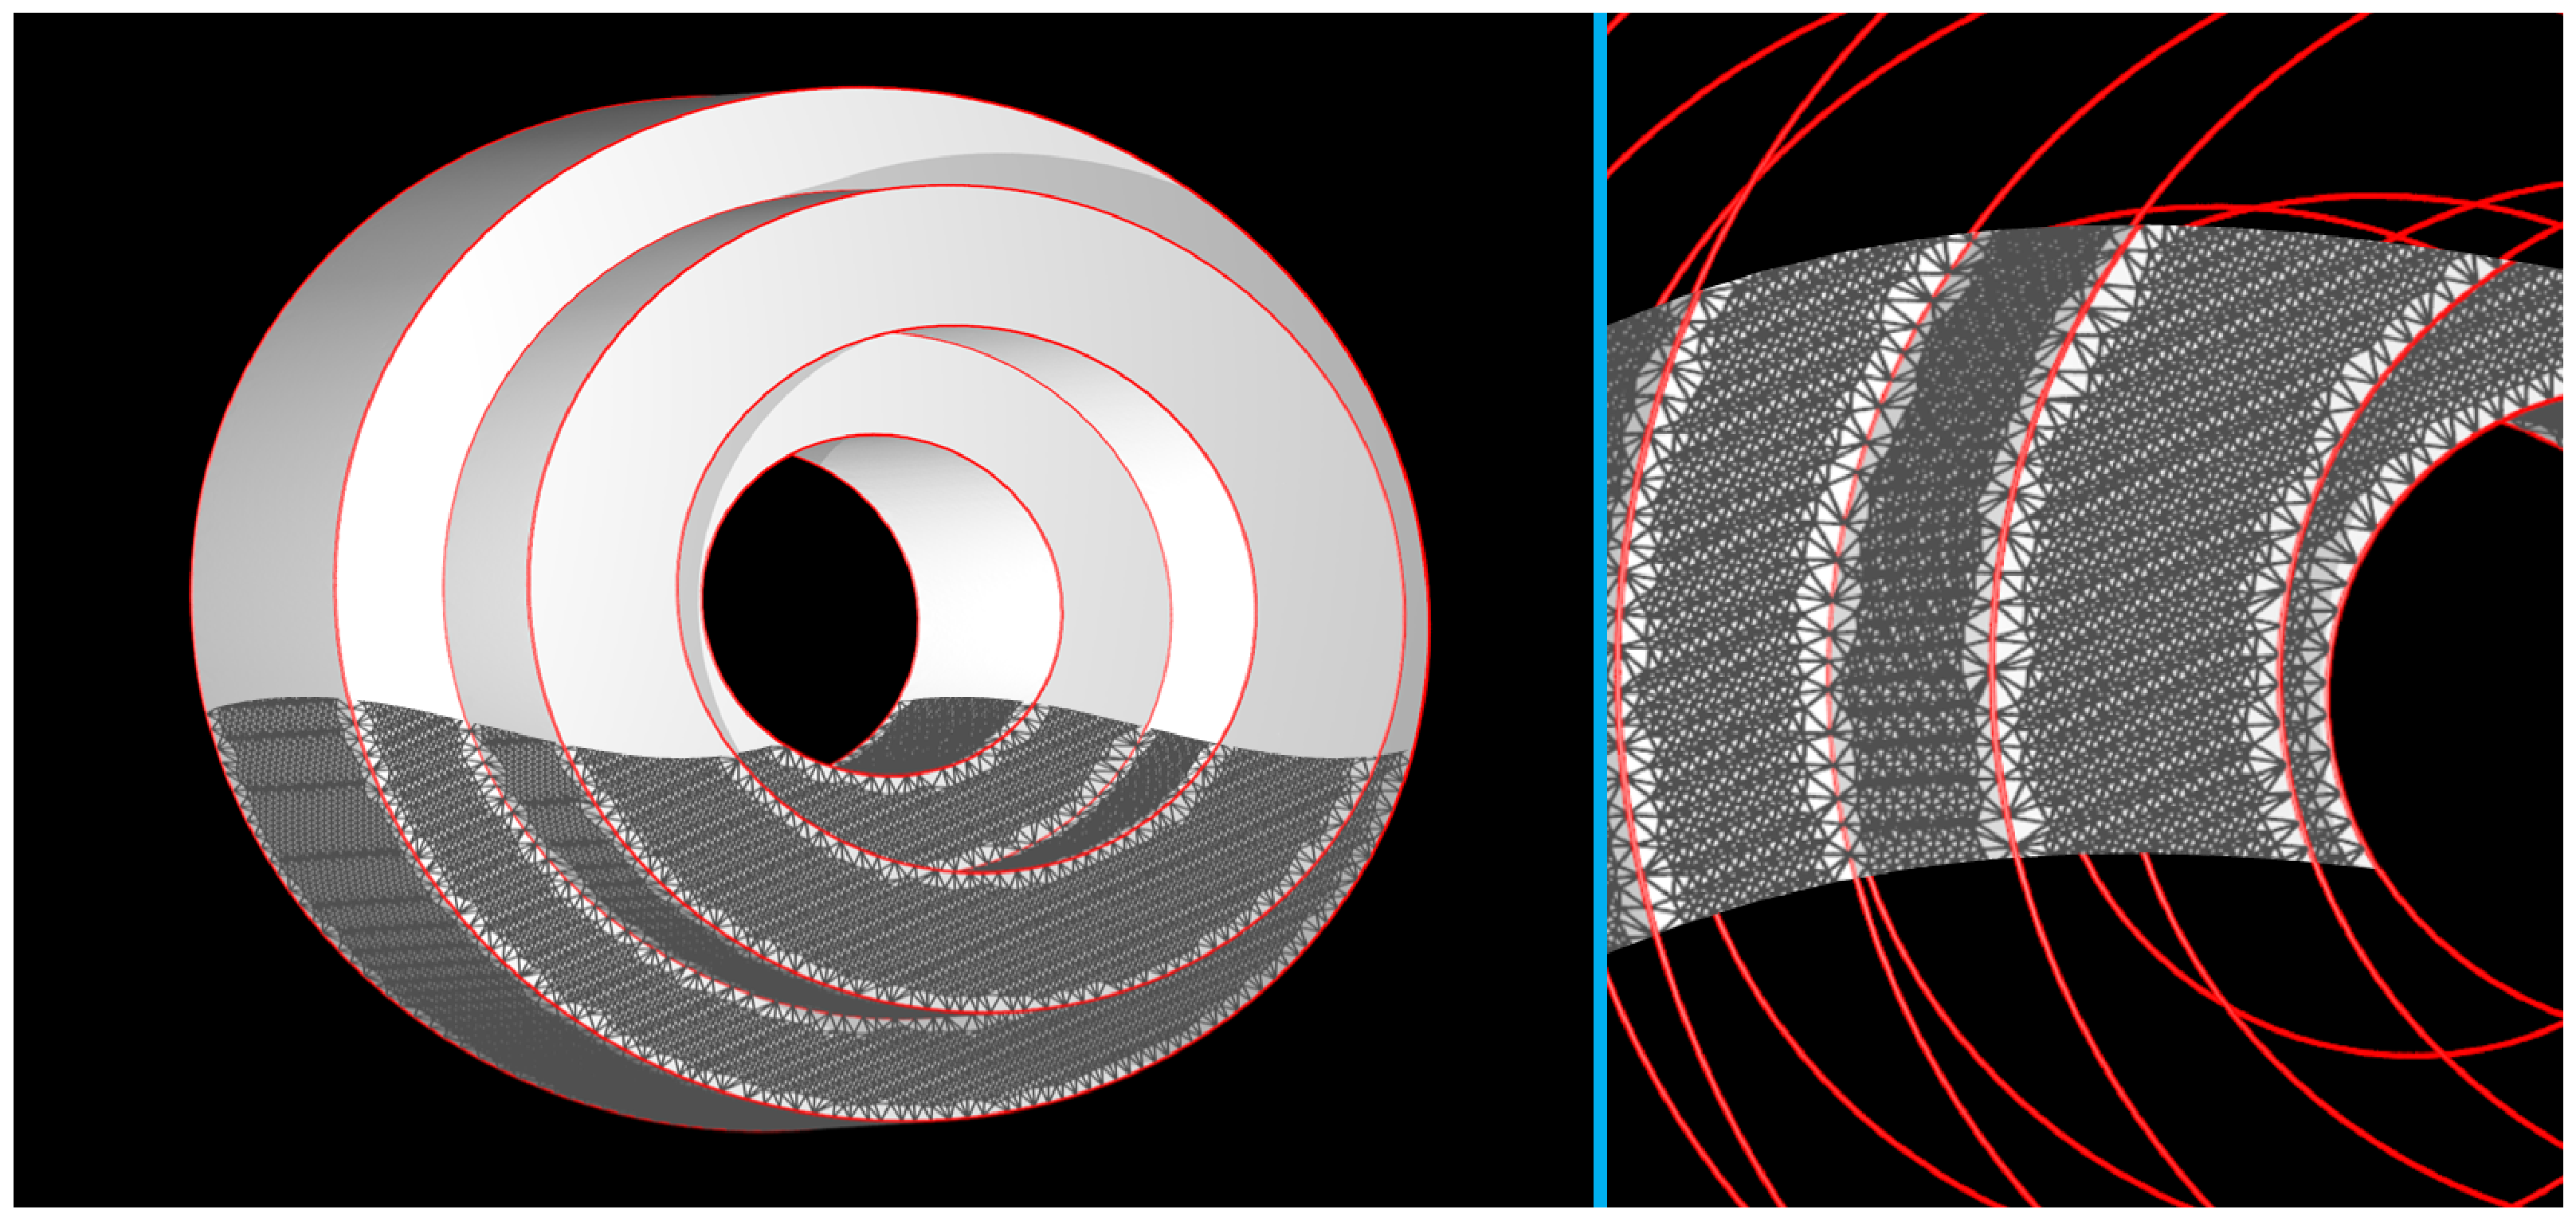
\includegraphics[width=\linewidth]{images/shrecFlangeCombine2.eps}
\caption{Result of SHREC on a Flange dataset. The FindSharp edges are marked in red. 
	Smooth edges are dark grey. The magnified region shows a blend of the FindSharp edges with the mesh edges.}
\label{fig:flange1}
\end{figure}
	 
\begin{figure*}[ht] 
	\centering
	\subfloat[]{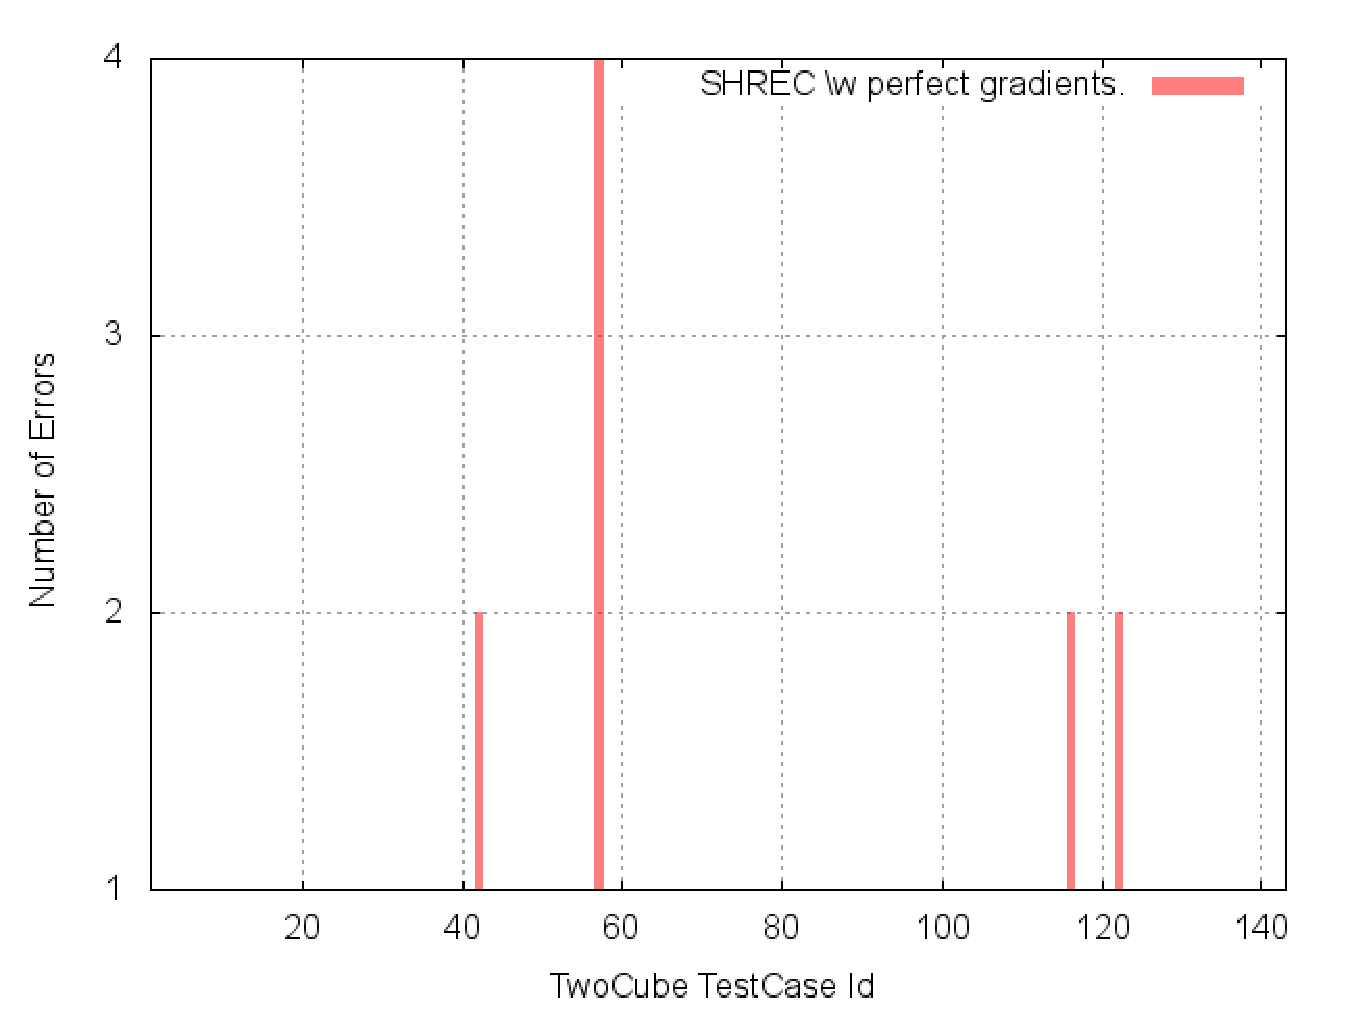
\includegraphics[width=0.24\linewidth]{images/shrecResCol1.eps}\label{fig:shrecTwoCube:a}}
	\subfloat[]{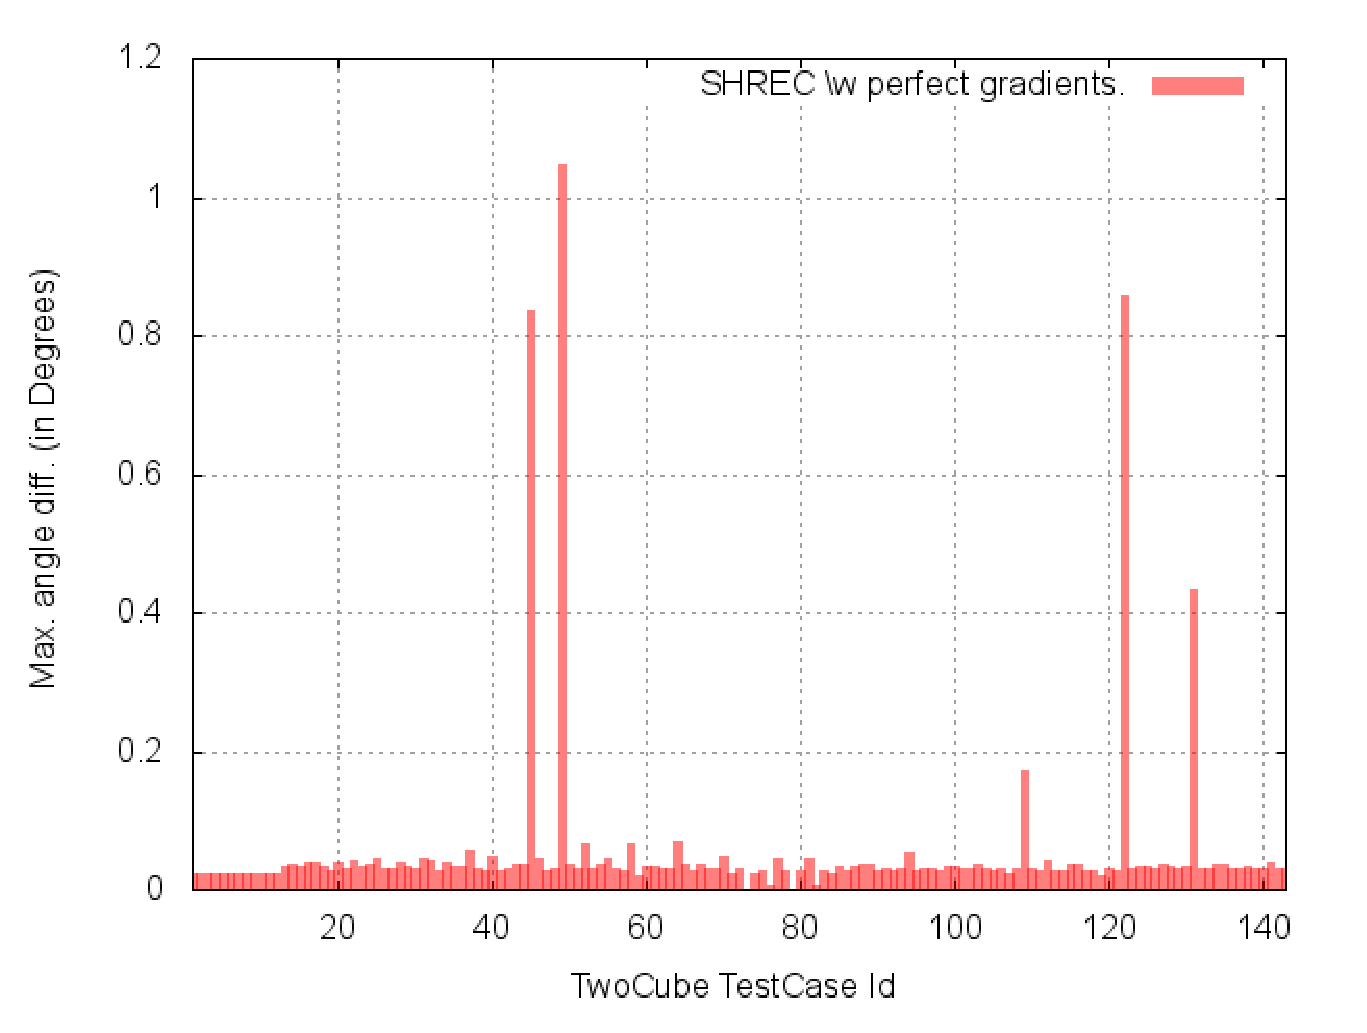
\includegraphics[width=0.24\linewidth]{images/shrecResCol3.eps}\label{fig:shrecTwoCube:b}}
	\subfloat[]{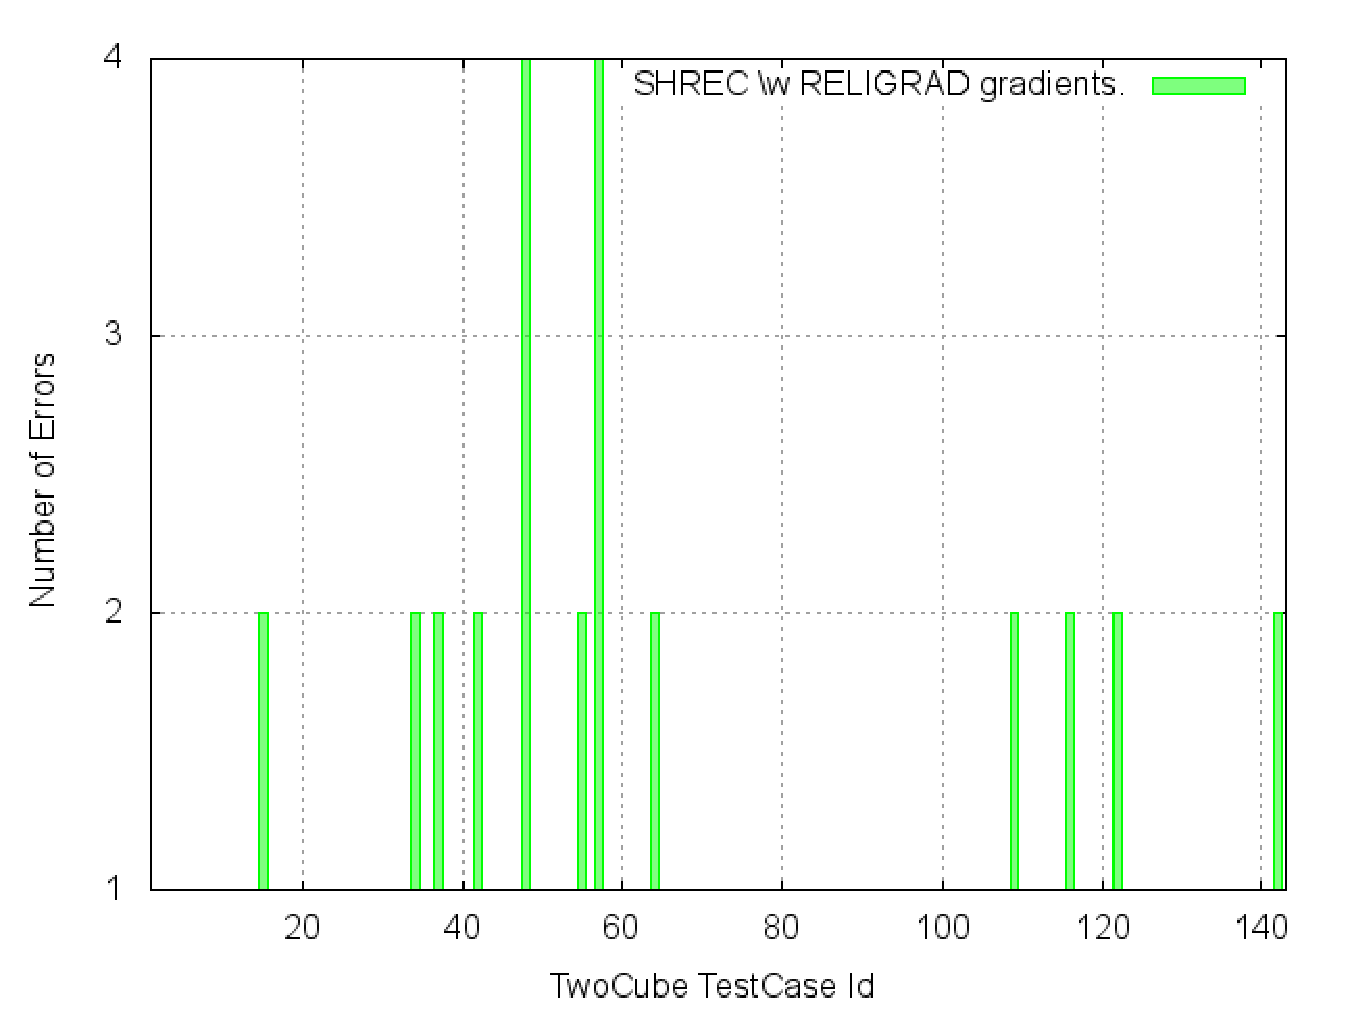
\includegraphics[width=0.24\linewidth]{images/shrecResCol2.eps}\label{fig:shrecTwoCube:c}}
	\subfloat[]{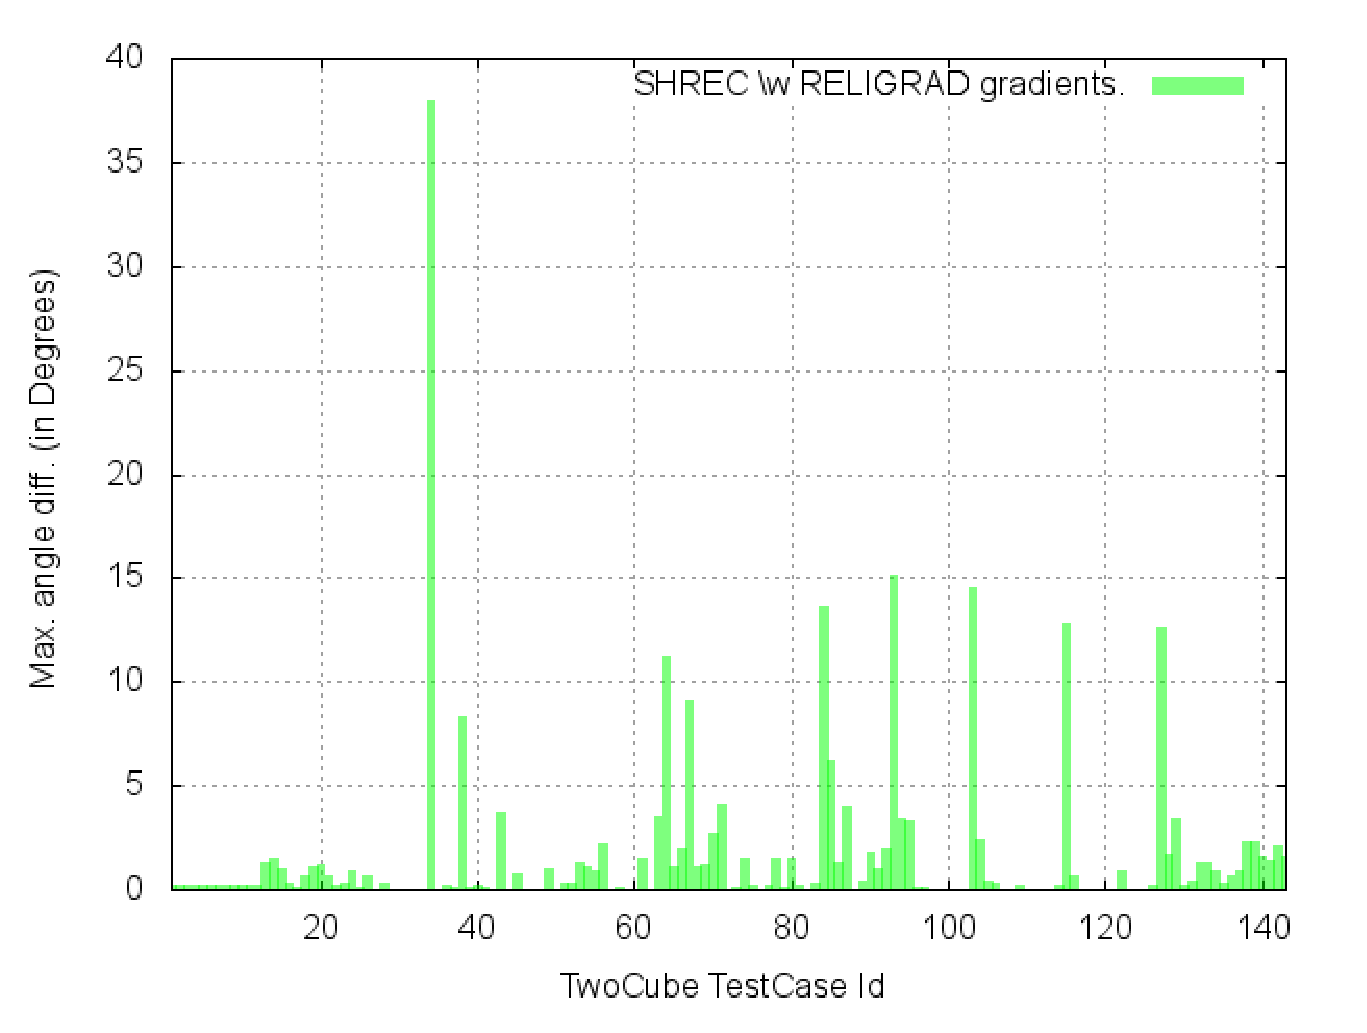
\includegraphics[width=0.24\linewidth]{images/shrecResCol4.eps}\label{fig:shrecTwoCube:d}}
	\caption{Shrec with perfect gradients and RELIGRAD (computing gradients from scalar data.) }
	\label{fig:shrecTwoCube}
	\vskip-0.2cm
\end{figure*}
Figure~\ref{fig:shrecTwoCube} shows the summary results on 143 TwoCube datasets. Figure~\protect\subref*{fig:shrecTwoCube:a} shows the number of CountDegree errors using the SHREC algorithm along with perfect gradients as inputs. Only four test cases have errors, with the maximum having four errors. 
Figure~\protect\subref*{fig:shrecTwoCube:b}, shows the maximum angle difference from the original mesh. The maximum angle difference is 1.05 degrees for the dataset id 50.

Figure~\protect\subref*{fig:shrecTwoCube:c}, shows the CountDegree results using SHREC with gradients generated from the scalar grid using RELIGRAD. The maximum number of errors for a single dataset is four. Figure~\protect\subref*{fig:shrecTwoCube:d} shows the maximum angle difference from the original perfect mesh. While the maximum error was 38 degrees for a single test, majority produced very small errors. Figure~\ref{fig:shrecPerfect1} shows the mesh and the edges generated on a particular dataset.

Figure~\protect\subref*{fig:cannon:a},~\protect\subref*{fig:cannon:b} show our results of running SHREC with RELIGRAD on the Cannon datasets. Figure~\protect\subref*{fig:cannon:b} shows the CountDegree errors generated for the 15 cannon sets using gradients computed from RELIGRAD. The maximum error generated was 2. SHREC on the perfect gradient generated 'NO' errors. Figure~\protect\subref*{fig:cannon:a} shows one representative result using SHREC and RELIGRAD directly from scalar data. The magnified region shows a portion of the sharp edge. 
\begin{figure}[tb]
	\includegraphics[width=\linewidth]{images/shrecperfect.eps}
	\caption{Result of SHREC on a twoCube dataset. The FindSharp Edges are marked in red. Smooth edges are shown in cyan. The magnified region shows the output mesh edges around a corner.}
	\label{fig:shrecPerfect1}
\end{figure}
\begin{figure}[tb]
	\subfloat[]{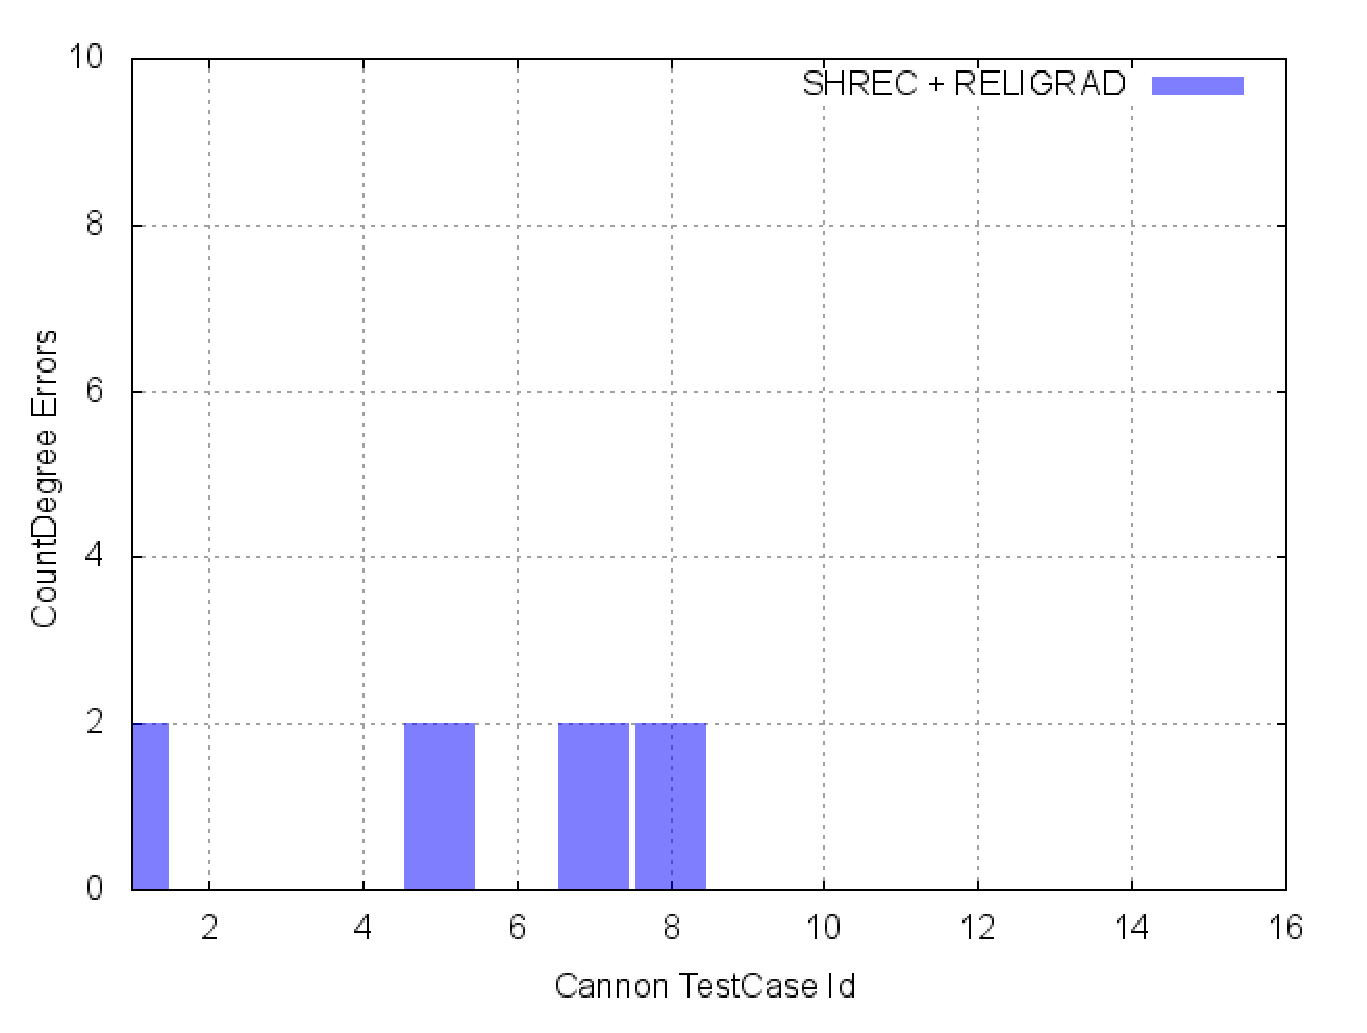
\includegraphics[width=0.5\linewidth]{images/cannon.eps}\label{fig:cannon:b}}
	\subfloat[]{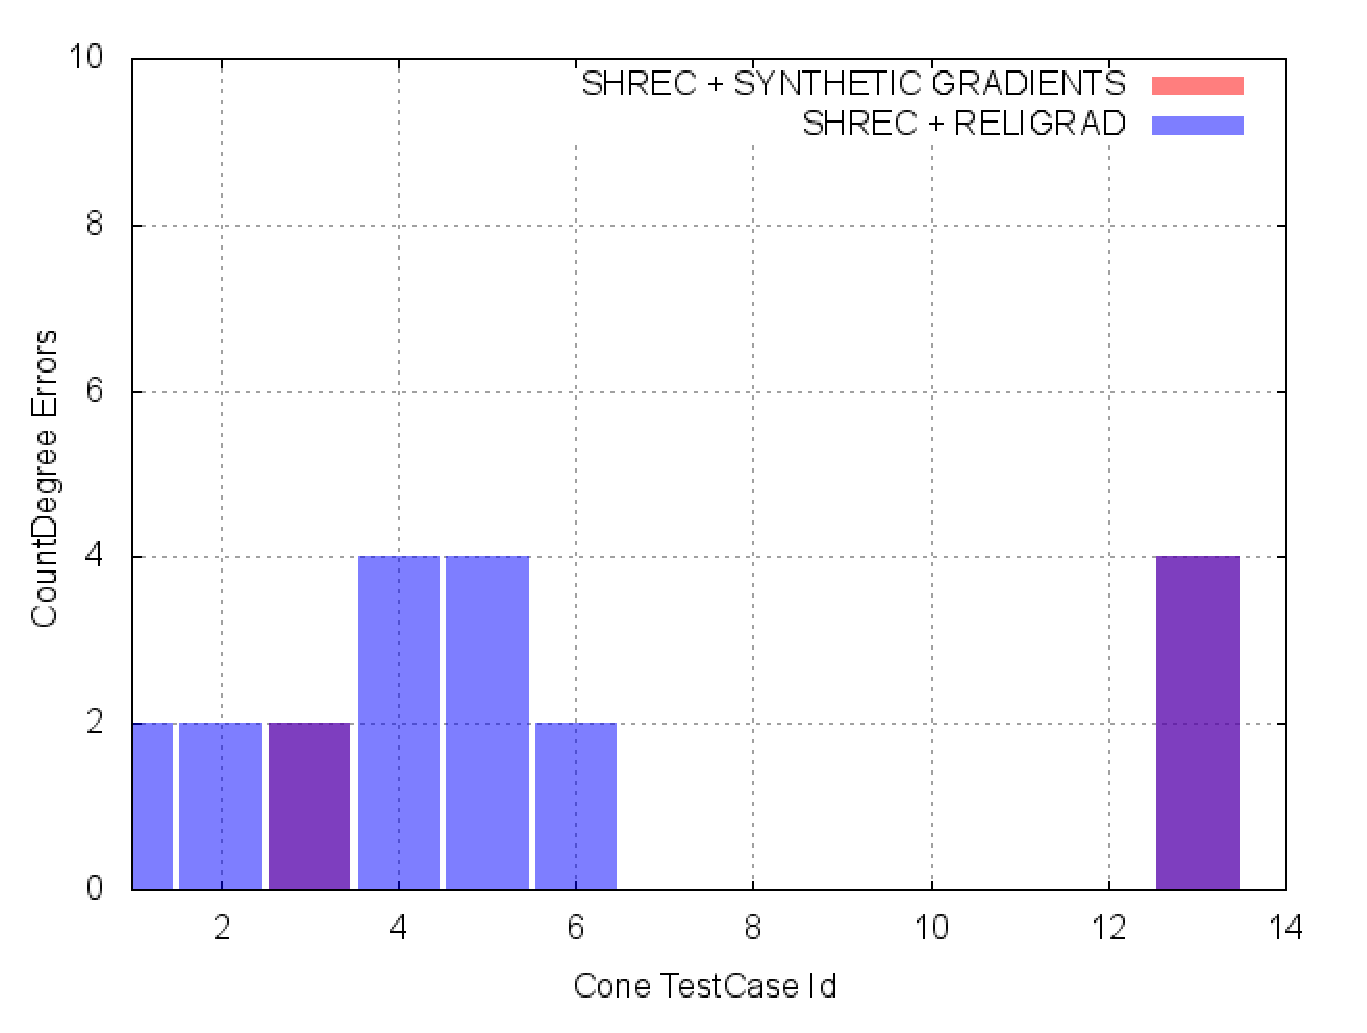
\includegraphics[width=0.5\linewidth]{images/cone.eps}\label{fig:cone:b}}
	\caption{Summary result of algorithm SHREC on Cannon and cone Datasets. (a) CountDegree Errors on 15 Cannon datasets using RELIGRAD gradients. SHREC with perfect gradients had no errors and is not shown. (b) CountDegree errors on 14 Cone datasets using RELIGRAD and perfect gradients.}
	\label{fig:cannon_cone_summary}
\end{figure}
\begin{figure}[tb]
	\subfloat[]{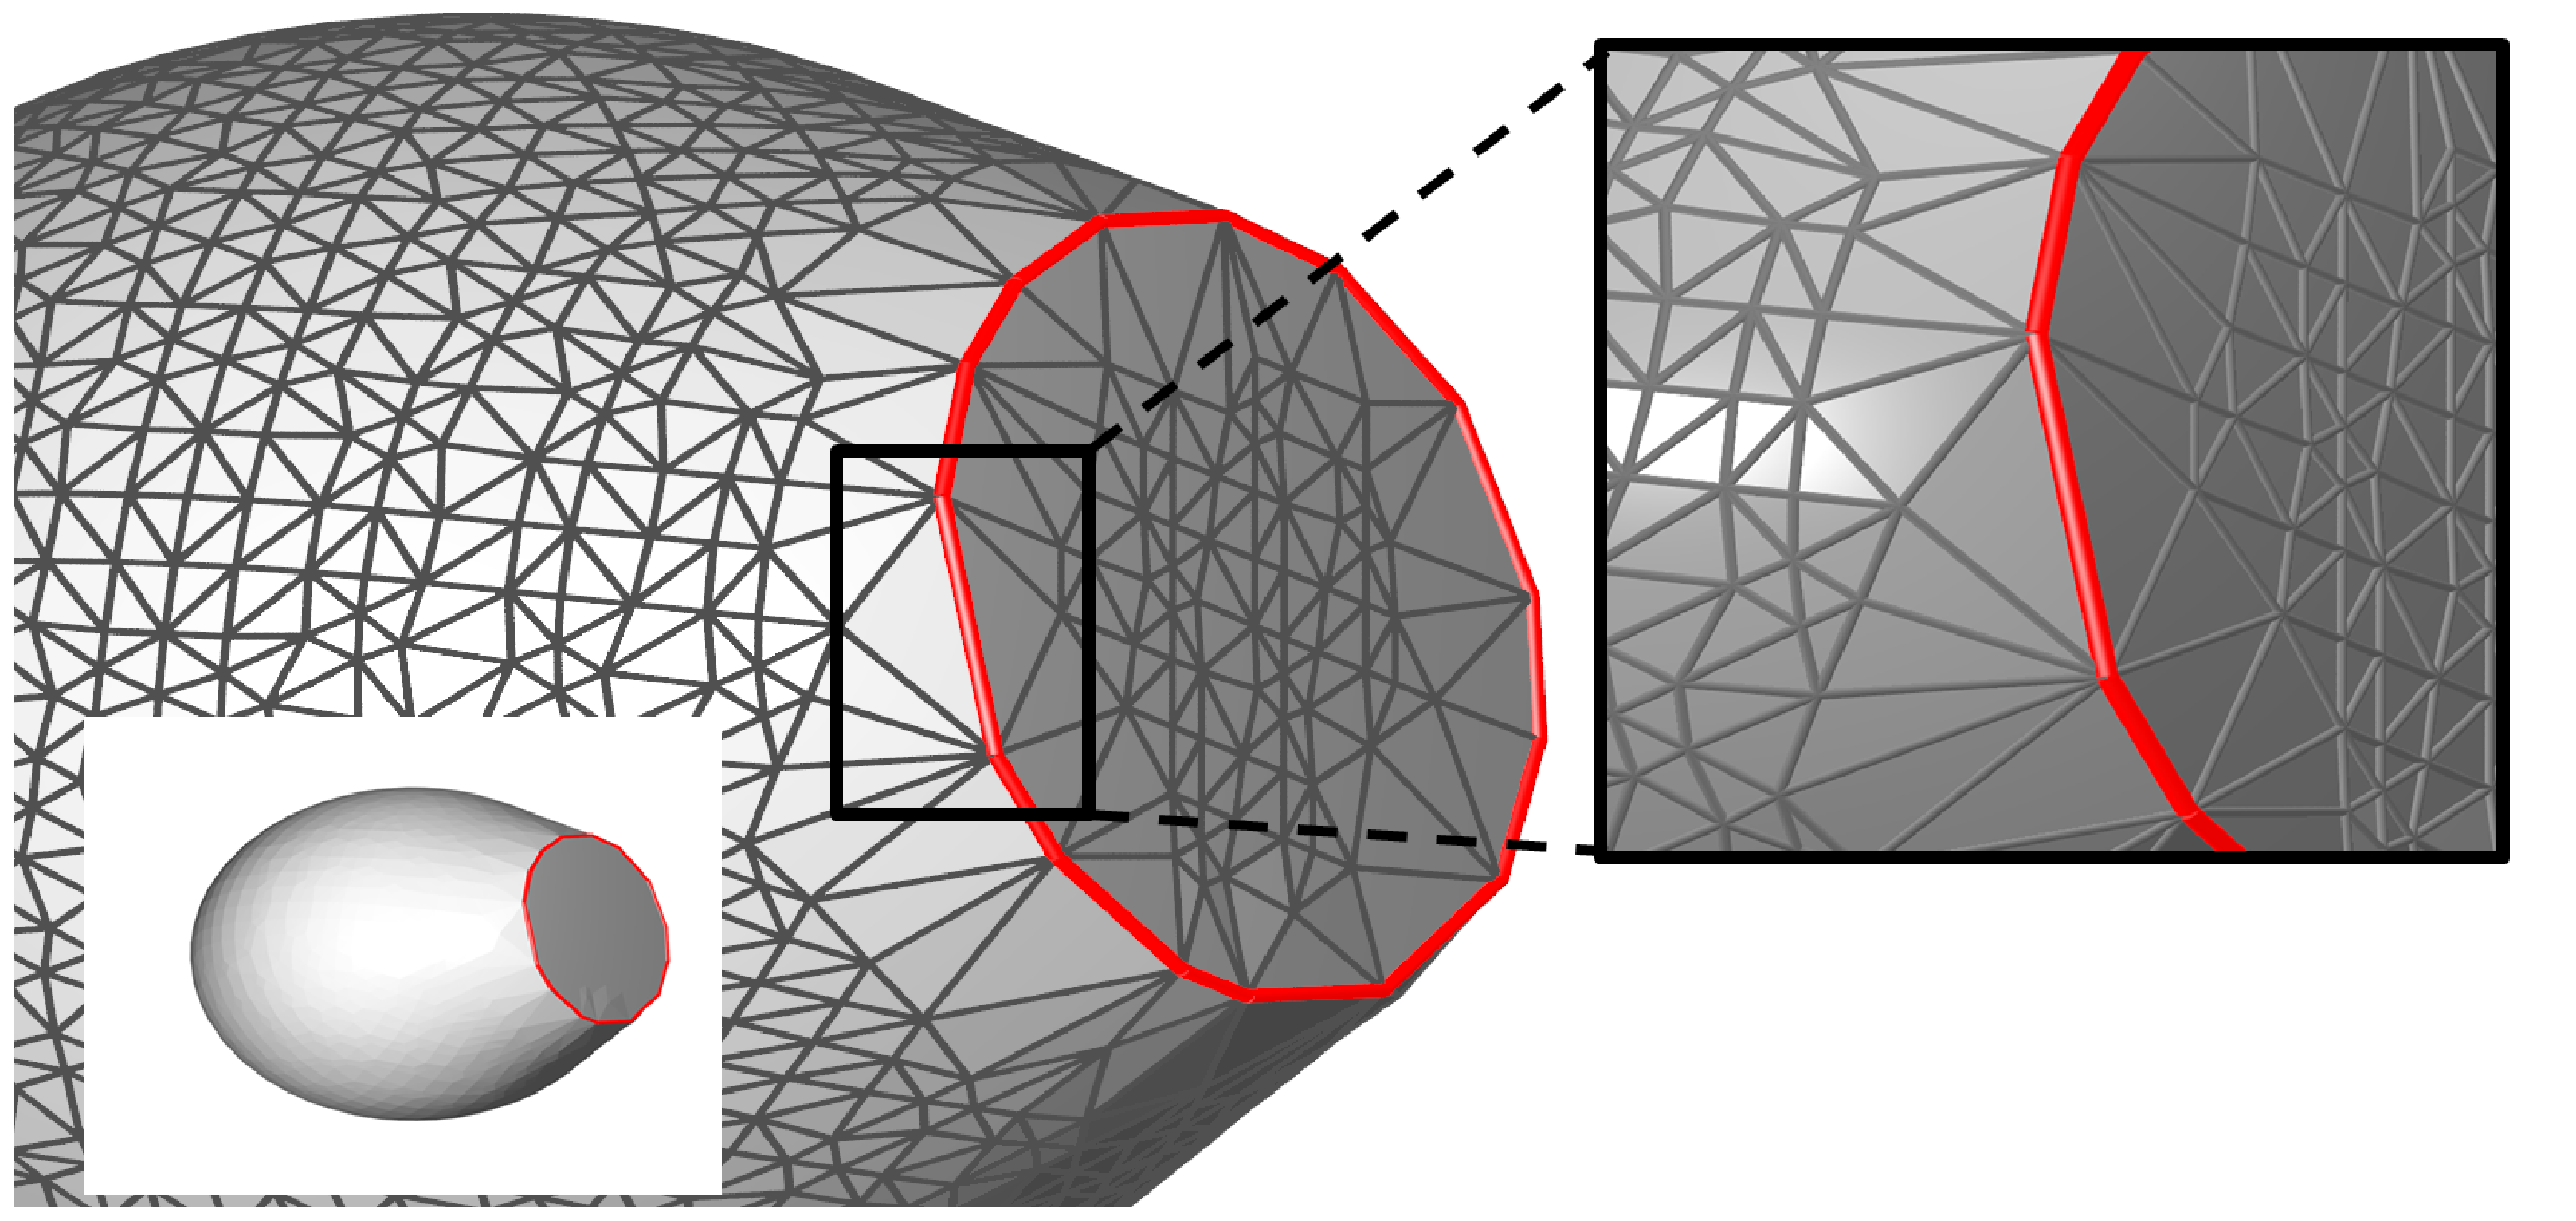
\includegraphics[width=0.5\linewidth]{images/cannon2.eps}\label{fig:cannon:a}}
	\subfloat[]{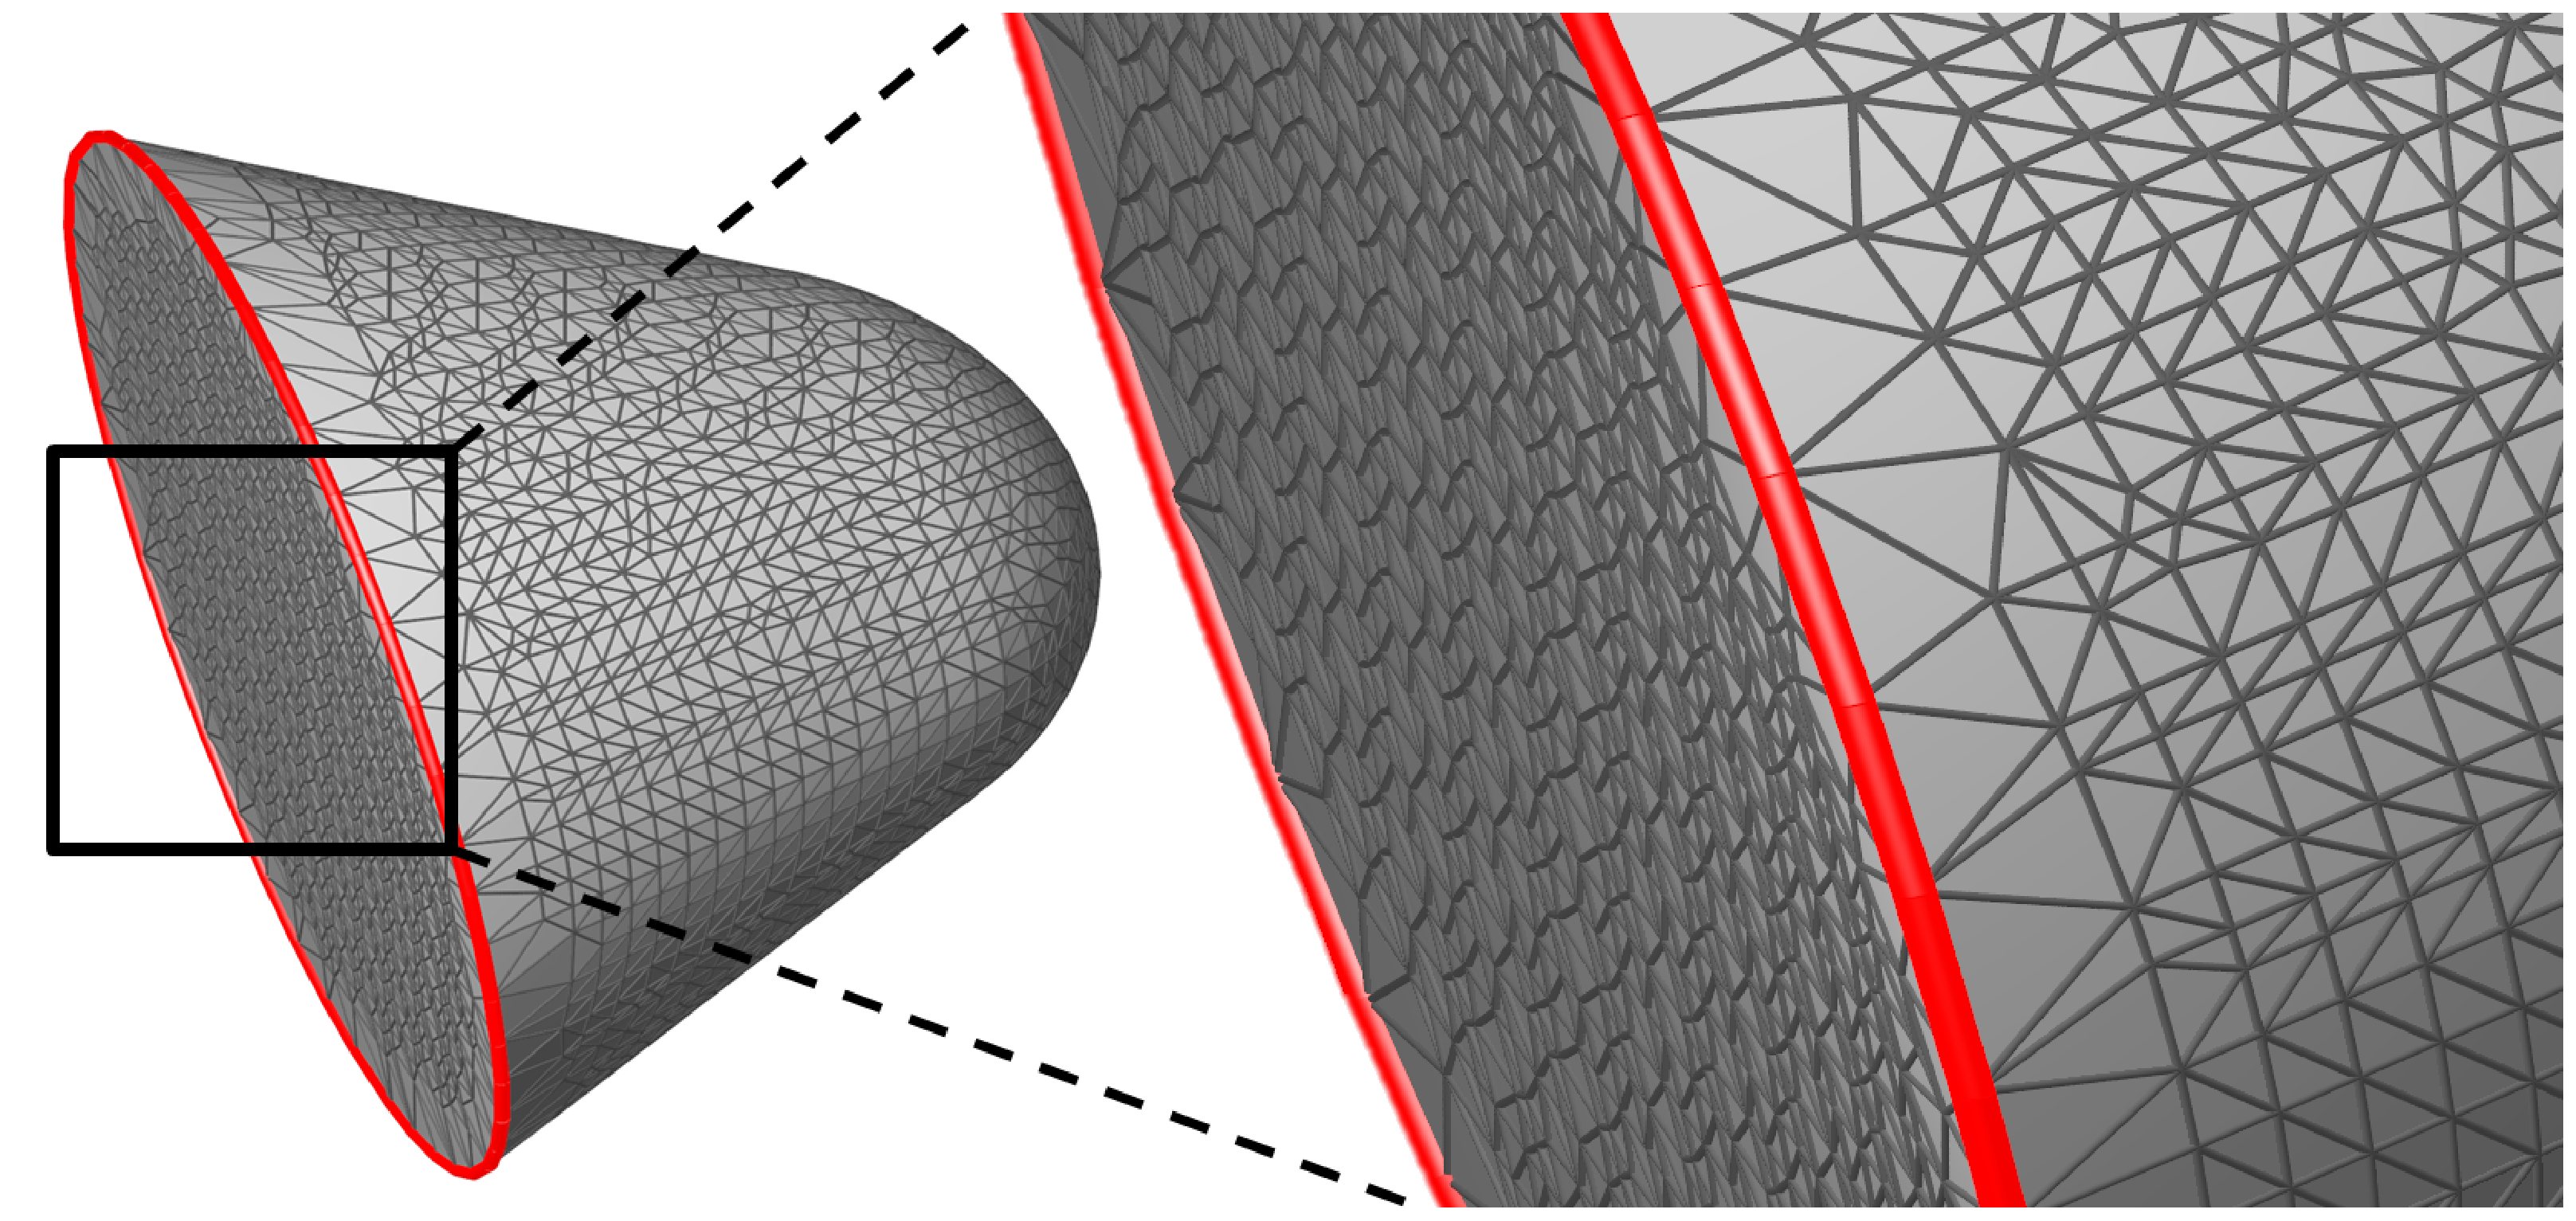
\includegraphics[width=0.5\linewidth]{images/cone2.eps}\label{fig:cone:a}}
	\caption{Result of algorithm SHREC with RELIGRAD gradients on Cannon and Cone datasets}
	\label{fig:cannon_cone}
\end{figure}
\section{Experimental Results on CT Data}

\subsection{Description of CT Data Sets}

\subsection{Comparison with Other Algorithms}
\paragraph{Comparison with Cocone}
We compare our algorithm to the algorithm WeightCocone by Dey et al.~\cite{Dey2012}. WeightCocone reconstructs a surface with sharp edges and corners from a sampled point cloud. WeightCocone takes two inputs; one contains the point cloud, another is a weighted sampling of feature curves. Weight of the sampling will be used as weight of the protecting balls. WeightCocone generates as output a feature sensitive mesh. 

The feature curve (second input to WeightCocone) is constructed using the algorithm FeatureRecon by Dey et al.~\cite{Dey2013}. FeatureRecon extracts feature curves of a surface. The input is a point cloud sampled on the surface. FeatureRecon has two steps, feature point detection and feature curves reconstruction. 

\textit{Experimental details:} The input to FeatureRecon is a point cloud. We tested two different input point cloud;
\begin{enumerate}
	\item We applied Marching Cubes~\cite{lc-mchr3-87} on our datasets Sec.\ref{sec:synData}. The vertices of the mesh generated by the Marching Cubes algorithm are then super-sampled using the Monte Carlo point sampling, to generate a point cloud with approximately sixty-five thousand points.
	\item We super-sampled the ``perfect" meshes Sec.\ref{sec:synData}, to generate generate a point cloud with approximately sixty-five thousand points.
\end{enumerate}
The two different point clouds are used as input to FeatureRecon to extract the feature curves. 
FeatureRecon has nine separate parameters. Experimentally and also noted by the authors Dey et al.~\cite{Dey2013}, we found FeatureRecon to be heavily reliant on parameter fine tuning. We used the following parameter values for our TwoCube datasets, (as suggest by the authors Dey et al.~\cite{Dey2013}). 
$-t = 25,-fl = 0.04, -cl = 0.06, -dc = 0, -\rho3 = 0.32, -\rho1 = 0.0, -rc = 3$.

The feature curves generated using FeatureRecon along with the super-sampled point cloud is used as input to WeighCocone. For comparison test, we compare the known ``perfect" mesh with the output of WeightCocone. 

We report both angular distance results and the FindSharp results.
\begin{figure}[t] 
	%dataset t110 reconstructed from perfect mesh 
	\centering  	
	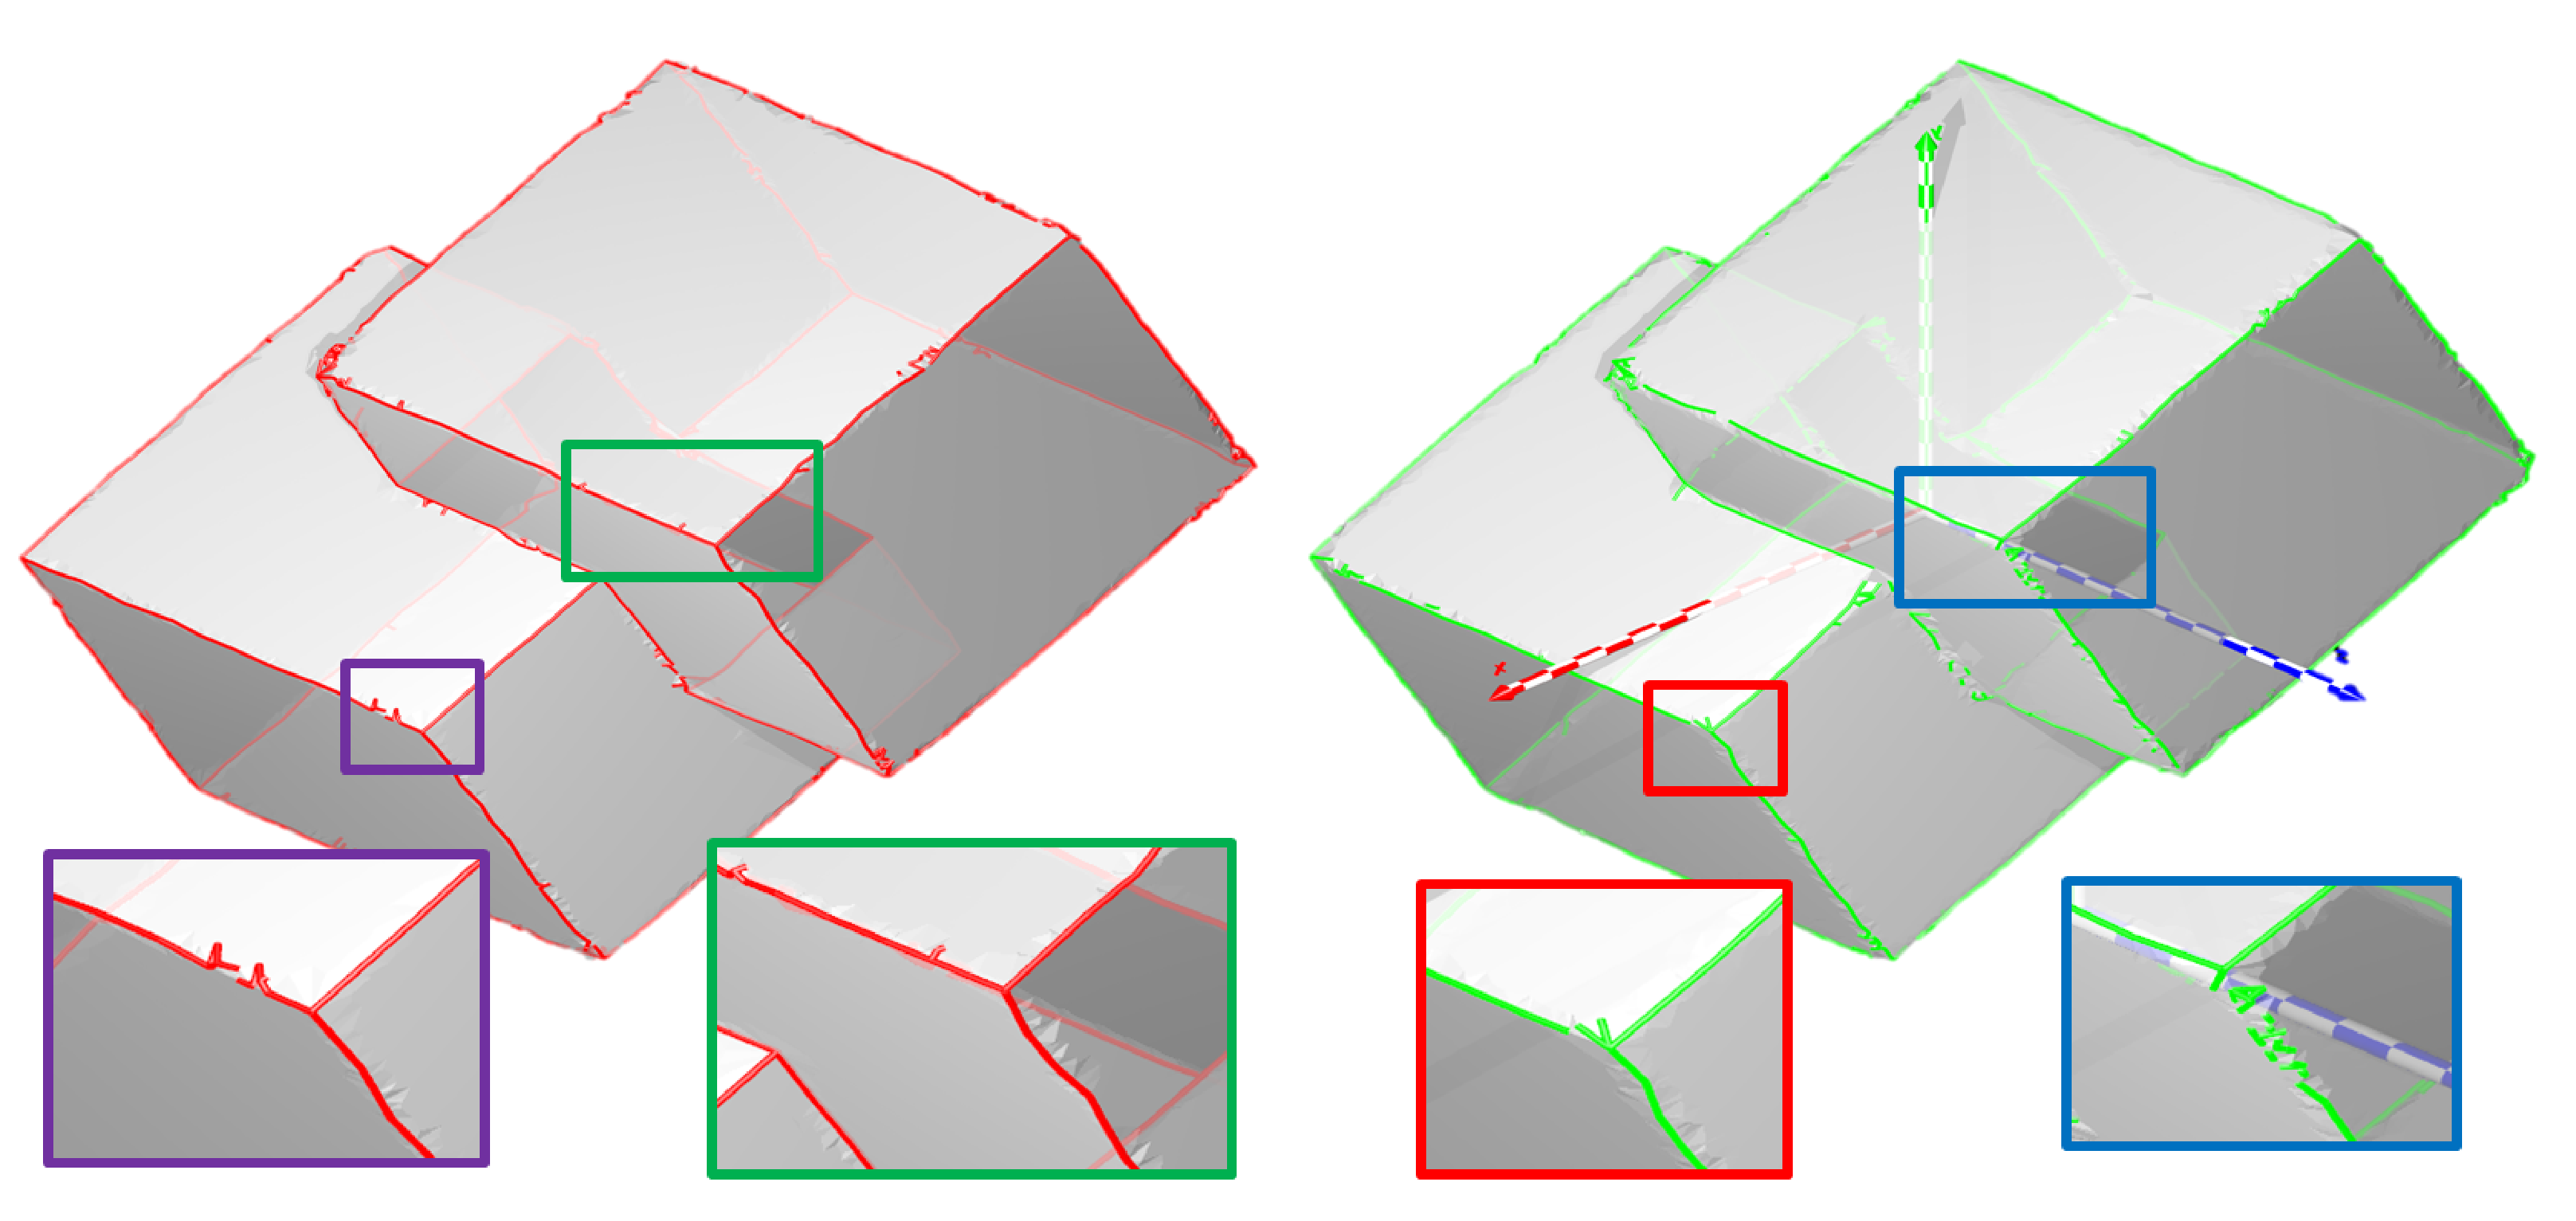
\includegraphics[width=\linewidth]{images/compare_cocone_perfect_mc.eps}
	\caption{Result of WeightCocone reconstruction on a TwoCube dataset (id 110). (a) Input cloud is the super-sampled ``perfect" mesh. (b) Input cloud is the super-sampled Marching Cube mesh. The magnified regions show some of the errors. The reconstruction from point cloud generated from the Marching Cube input is worse than the  point cloud from ``perfect" mesh input. }
	\label{fig:cocone_compare_from_perfect_1}
	\vskip-0.2cm
\end{figure} 



Figure~\ref{fig:cocone_compare_from_perfect_1} shows the reconstructed mesh for dataset id 110. The associated FindSharp edges are also shown. Figure~\ref{fig:cocone_compare_from_perfect_1}(a) shows the reconstruction from the point cloud generated from the ``perfect" mesh (henceforth refereed to as WeightCocone:a). The overlay-ed FindSharp edges (in red) show that the reconstruction has many errors. The magnified regions show some of the errors along the sharp edges and corners. Figure.~\ref{fig:cocone_compare_from_perfect_1}(b) shows the reconstruction from the point cloud generated from running Marching Cubes(henceforth refereed to as WeightCocone:b). The magnified regions show the same regions as Figure.~\ref{fig:cocone_compare_from_perfect_1}(a). The reconstruction is worse than WeightCocone:a(Figure.~\ref{fig:cocone_compare_from_perfect_1}(a)).

Figure~\protect\subref*{table:cocone_compare_with_mc_table_2} shows the angular distance from the perfect mesh to those generated by WeightCocone:a over a randomly selected subset of 21 cases out of the 140 TwoCube datasets. We show the number of simplices with more than 30, 40 and 50 degree errors. Figure~\ref{fig:shrecTwoCube} shows that algorithm SHREC comparatively generates far fewer errors. WeightCocone:b which uses the Marching Cubes point cloud as input produces worse results than WeightCocone:a and is not shown.

Figure~\protect\subref*{table:cocone_compare_with_mc_table_1} shows the results on a single dataset, the same as in figure~\ref{fig:cocone_compare_from_perfect_1}. It shows the surface angle difference from the original mesh while using the three algorithms; WeightCocone:a, WeightCocone:b and SHREC. WeightCocone:a performs better than WeightCocone:b but still has considerable errors. SHREC on that dataset produces no errors (Figure~\ref{fig:shrecPerfect1}). 

Dey et al.~\cite{Dey2012,Dey2013} report better results on their datasets. Which might possibly be because of parameter tuning. They themselves acknowledged as such in their work.
\begin{figure}
		\subfloat[]{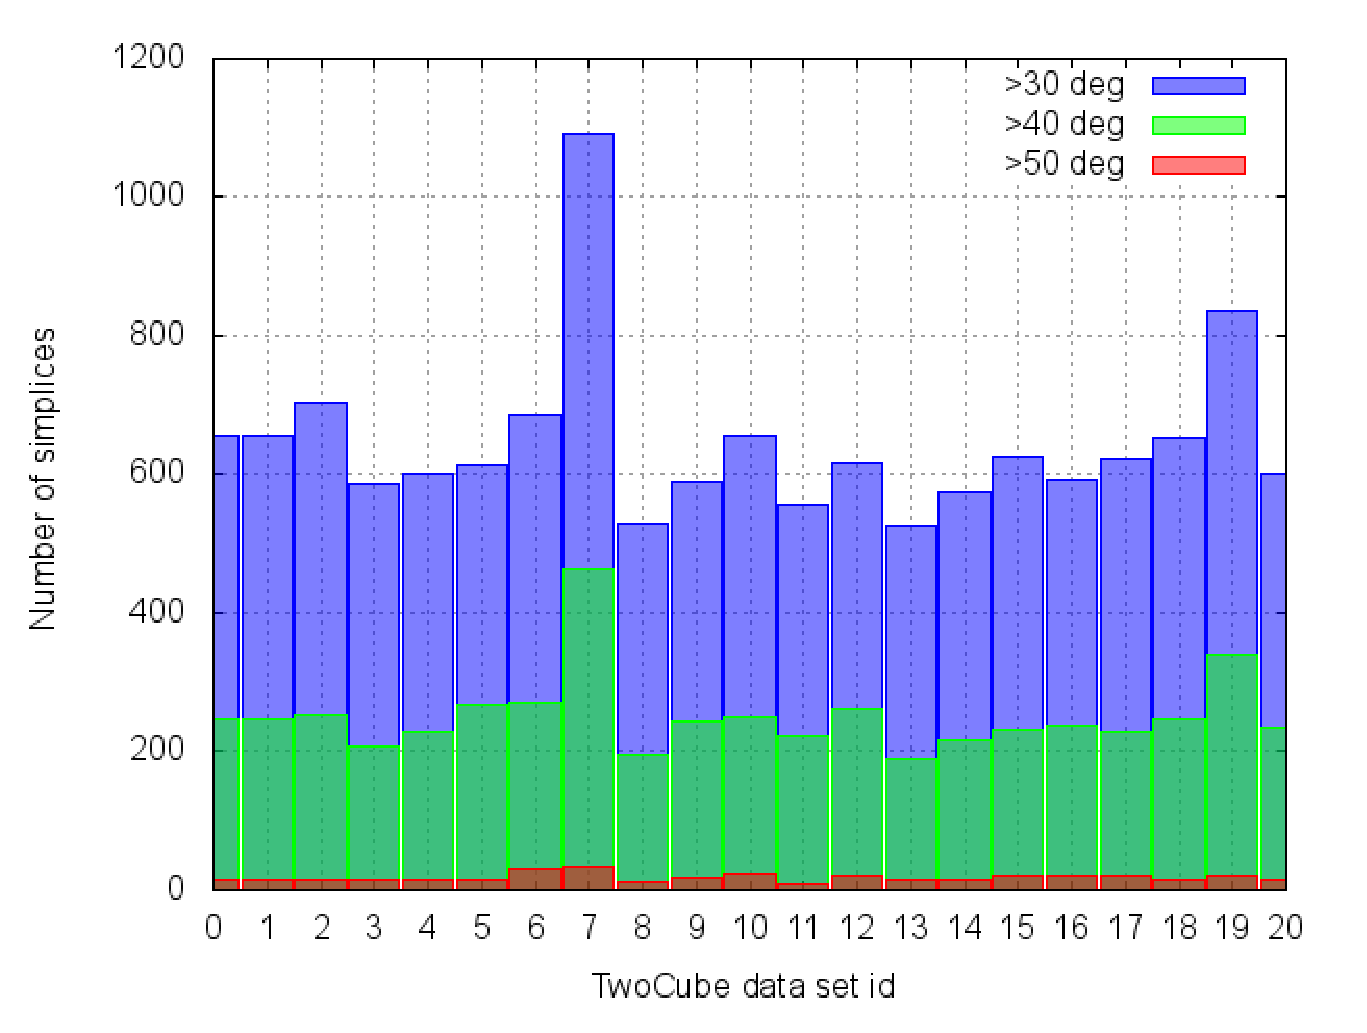
\includegraphics[width=0.5\linewidth]{images/num_simplices_large_test_twoCube.eps}\label{table:cocone_compare_with_mc_table_2}}
		\subfloat[]{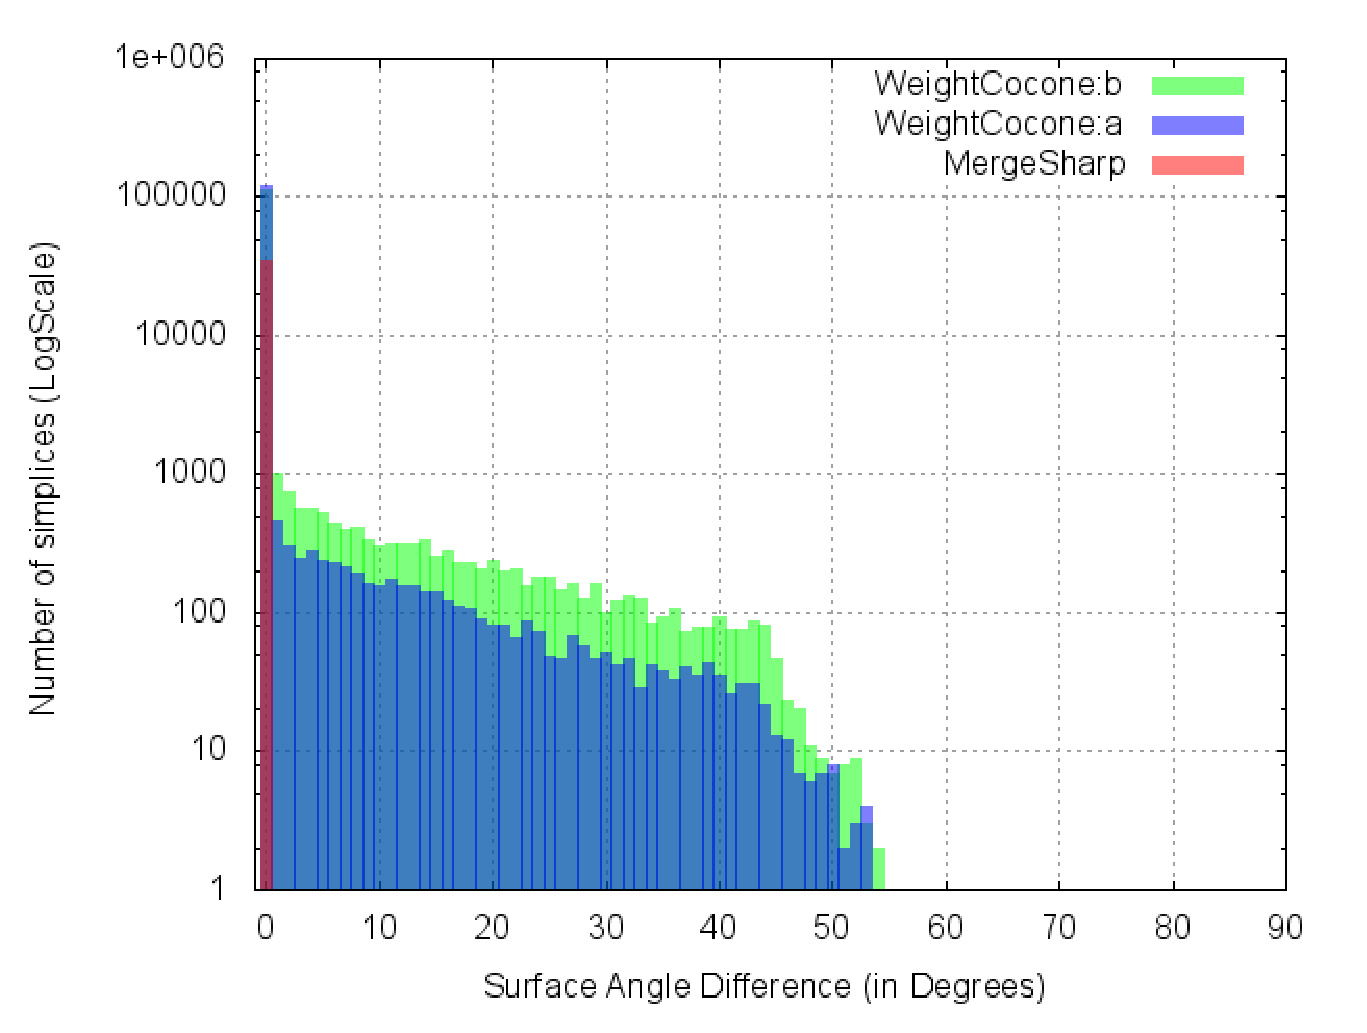
\includegraphics[width=0.5\linewidth]{images/num_simplices_histogram.eps}\label{table:cocone_compare_with_mc_table_1}}
		\caption{Cocone comparison Dey et al.~\cite{Dey2012,Dey2013}. (a) Number of simplices with angle difference of 30, 40 and 50 degrees from the original mesh on a subset of 21 TwoCube datasets using WeightCocone:a. (b) Number of simplices and the corresponding angle difference to the original mesh for a single TwoCube dataset, using WeightCocone:a, WeightCocone:b and SHREC.}
\end{figure}
\paragraph{Polymender comparison;}
We next compared SHREC to Polymender. Polymender is an implementation of mesh repairing algorithm from Ju~\cite{j-rrpm-04}. Figure~\protect\subref*{fig:polymender:b} shows the result of running Polymender on a flange dataset. Polymender creates creases, notches overlapping/degenerate triangles. On the same dataset SHREC with correct gradients and gradient computed from scalar data using RELIGRAD generates no errors, Figure~\protect\subref*{fig:polymender:a} shows the corresponding result. We quantitatively compare the surface angle difference between the Polymender and SHREC result with the known perfect mesh. 
The results in Figure~\protect\subref*{fig:polymender:c} shows the results. Polymender produces many simpices which have large angle difference from the perfect mesh. 
\begin{figure}[tb]
	\centering
		\subfloat[]{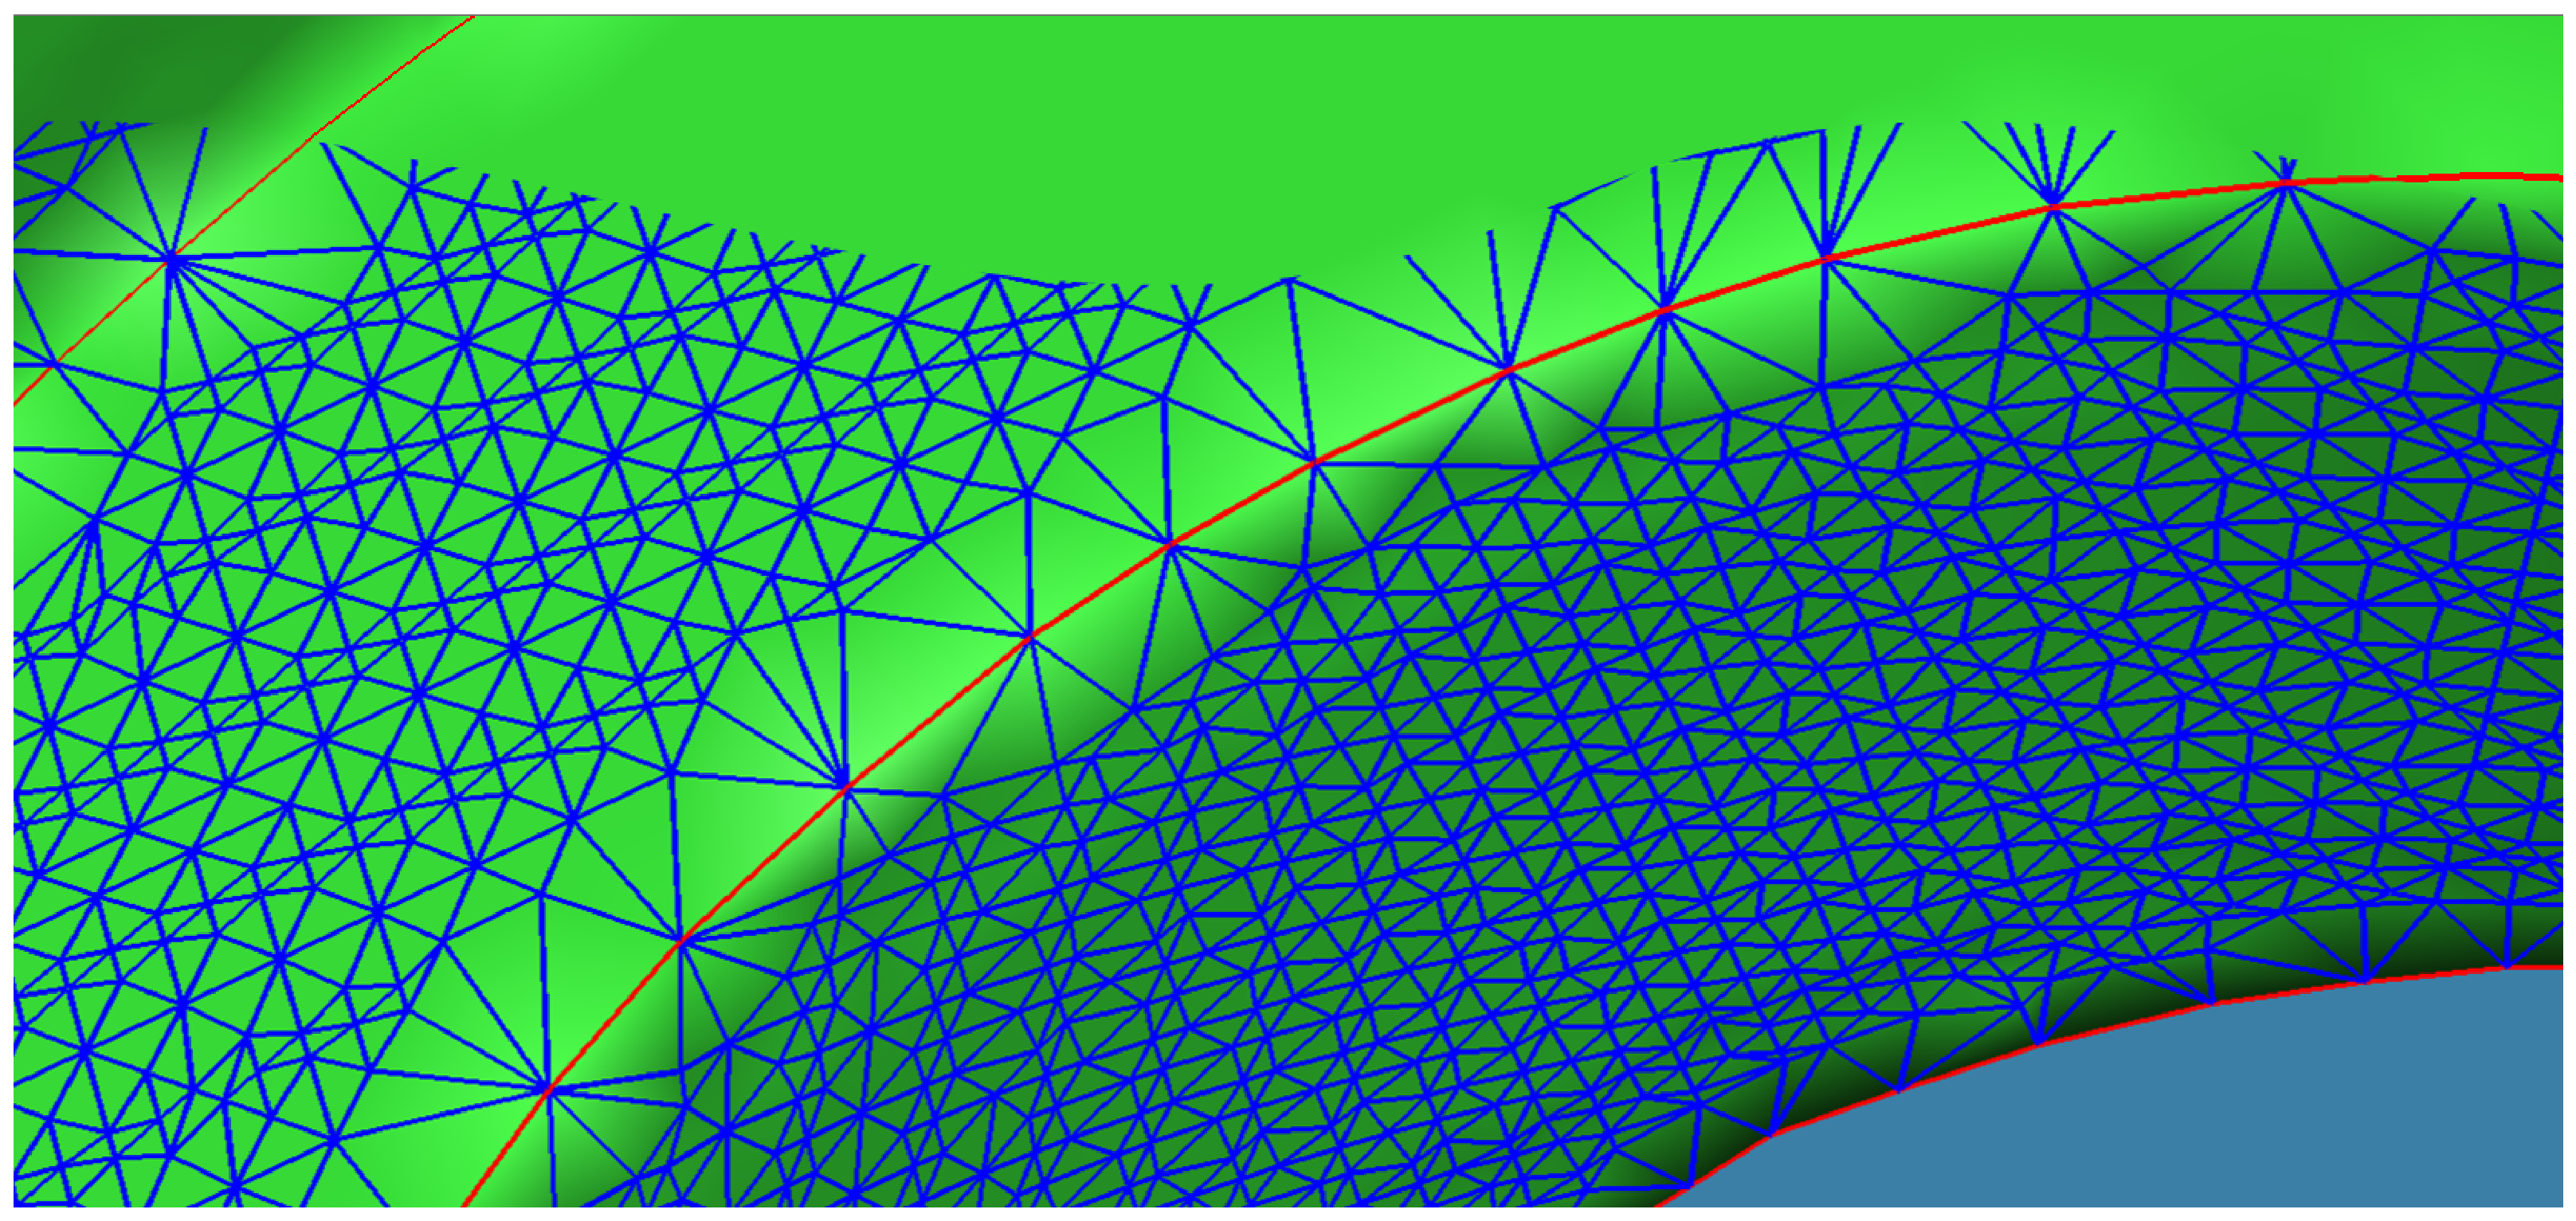
\includegraphics[width=\linewidth]{images/polymender3.eps}\label{fig:polymender:a} }\\
		\subfloat[]{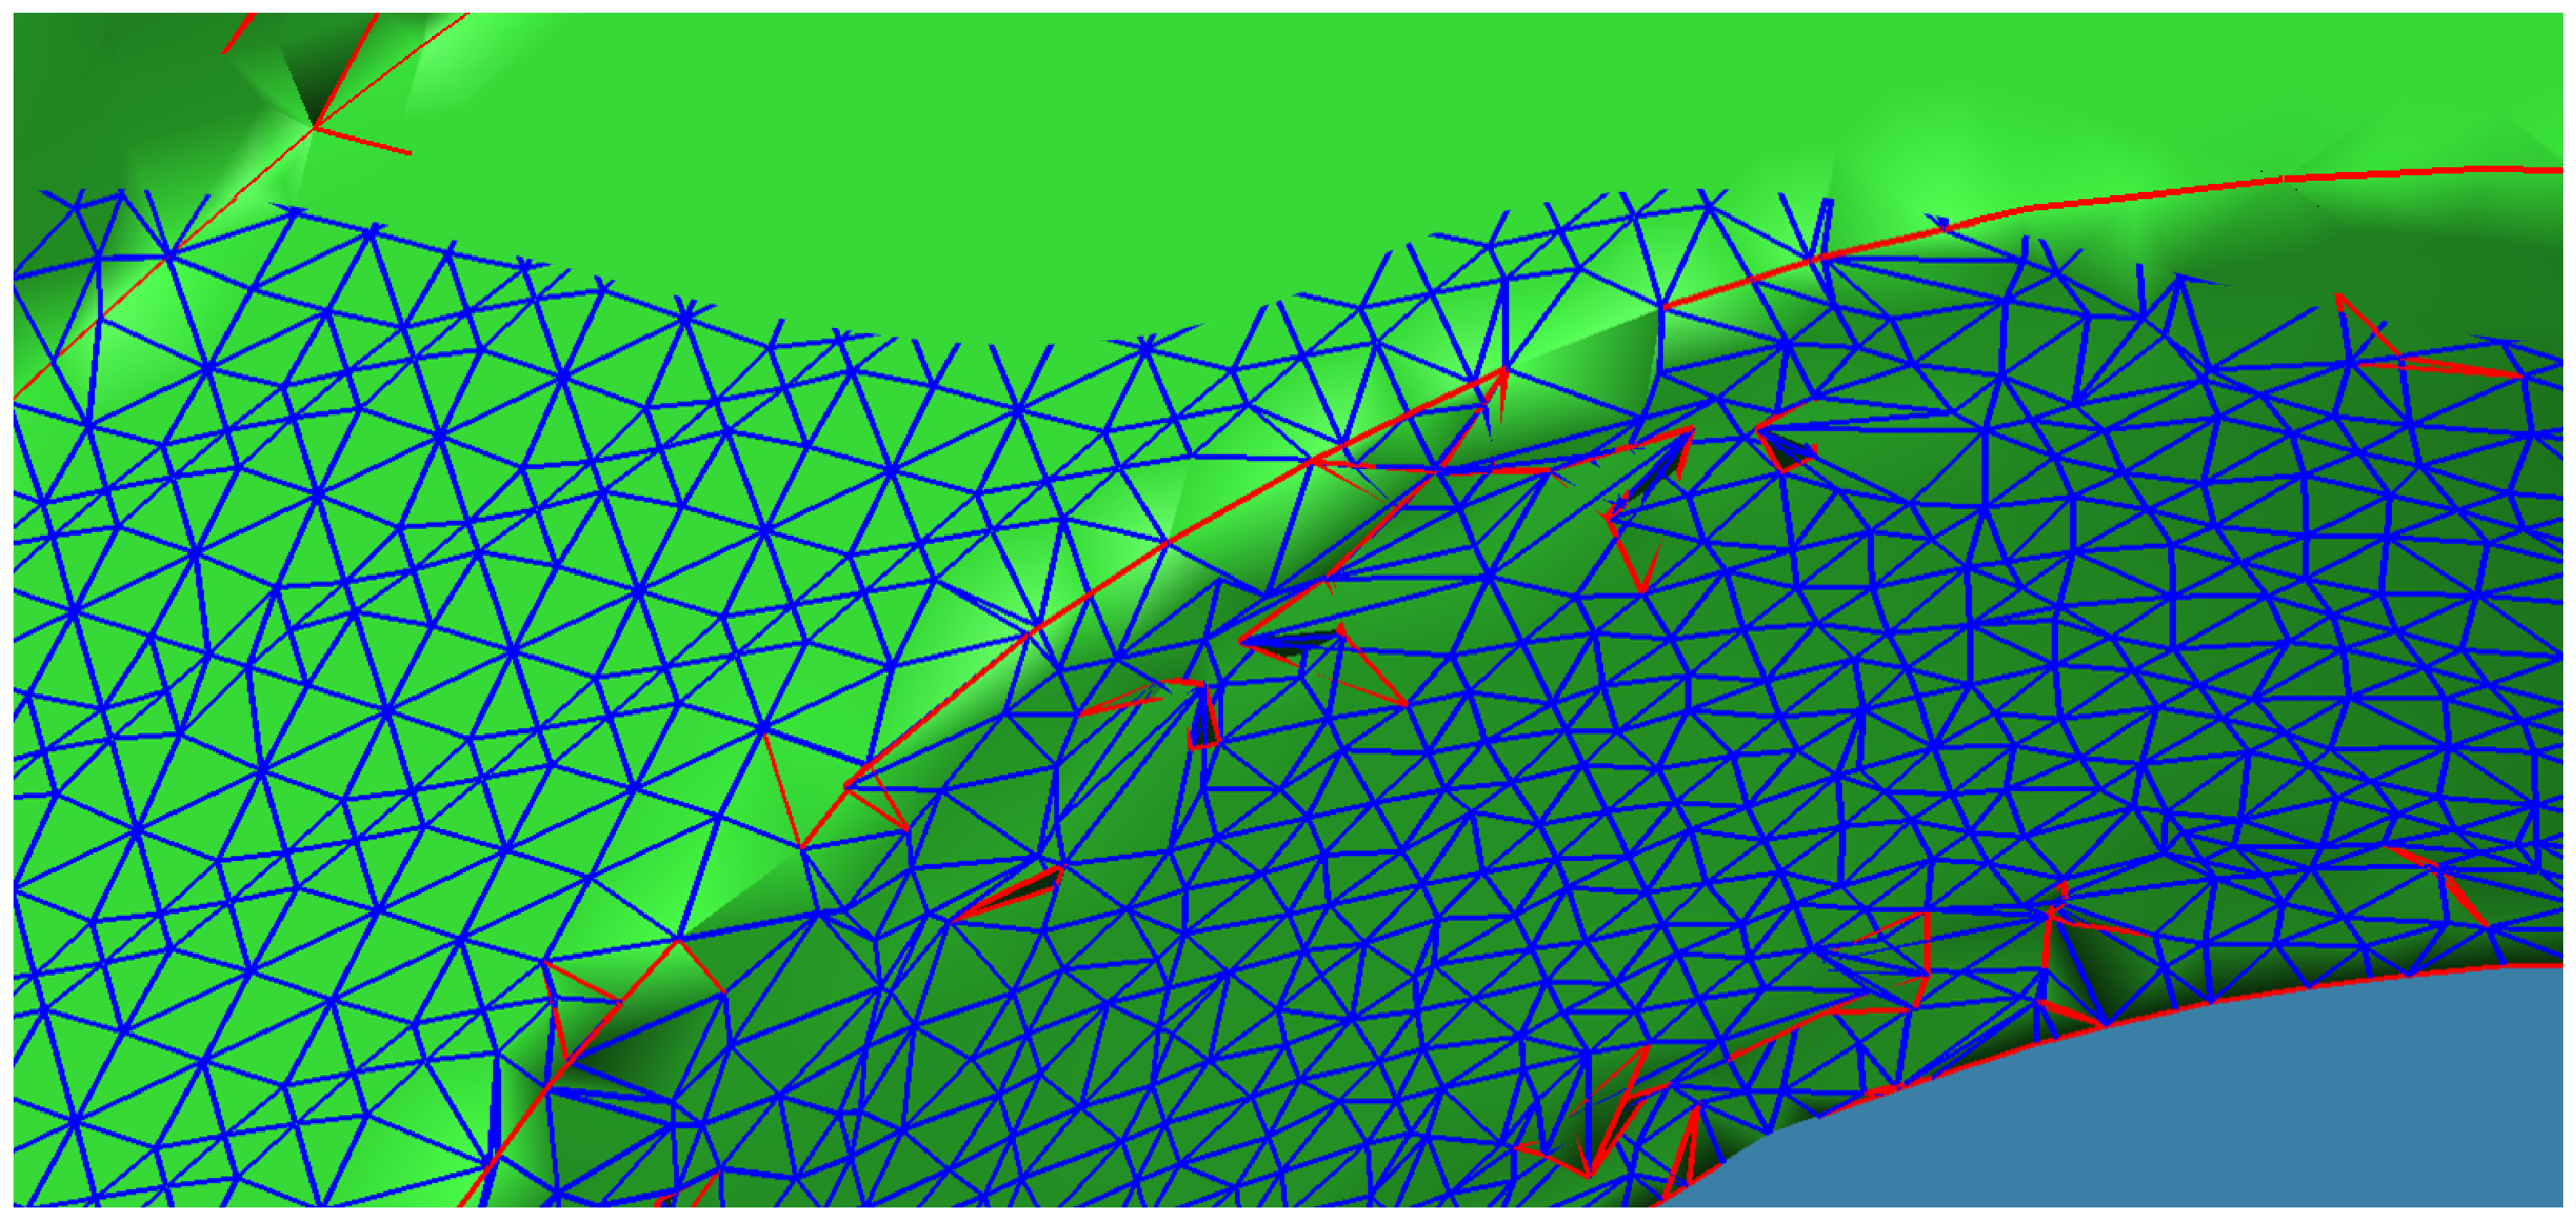
\includegraphics[width=\linewidth]{images/polymender4.eps}\label{fig:polymender:b}}\\
		\subfloat[]{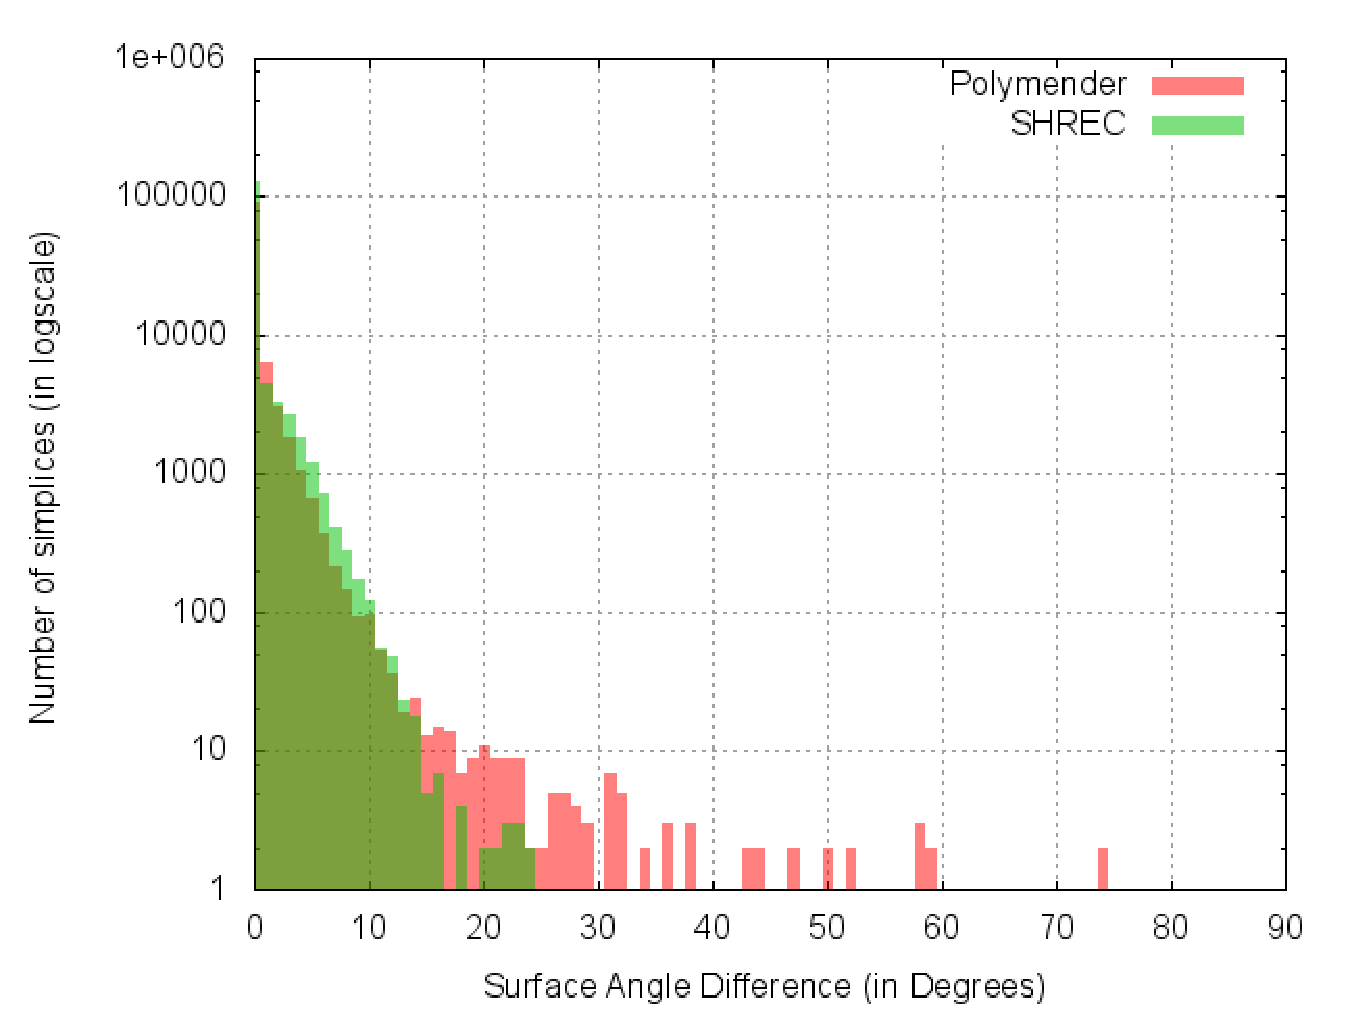
\includegraphics[width=\linewidth]{images/polymenderHistogram_1.eps}\label{fig:polymender:c}}
		\caption{Comparison of Polymender with SHREC on a Flange dataset. The edges with dihedral angle less than $140^\circ$ are overlay-ed in red, a subset of the rest of the edges are overlay-ed in blue. (a) SHREC with RELIGRAD on a part of a flange dataset. (b) Polymender on the same part. (c) Surface angle distance for the two results from the perfect mesh. Y-axis is in logscale. }	
\end{figure}
\paragraph{Extended Marching Cubes comparison;}
\begin{figure}[tb]
	\centering
	\subfloat[]{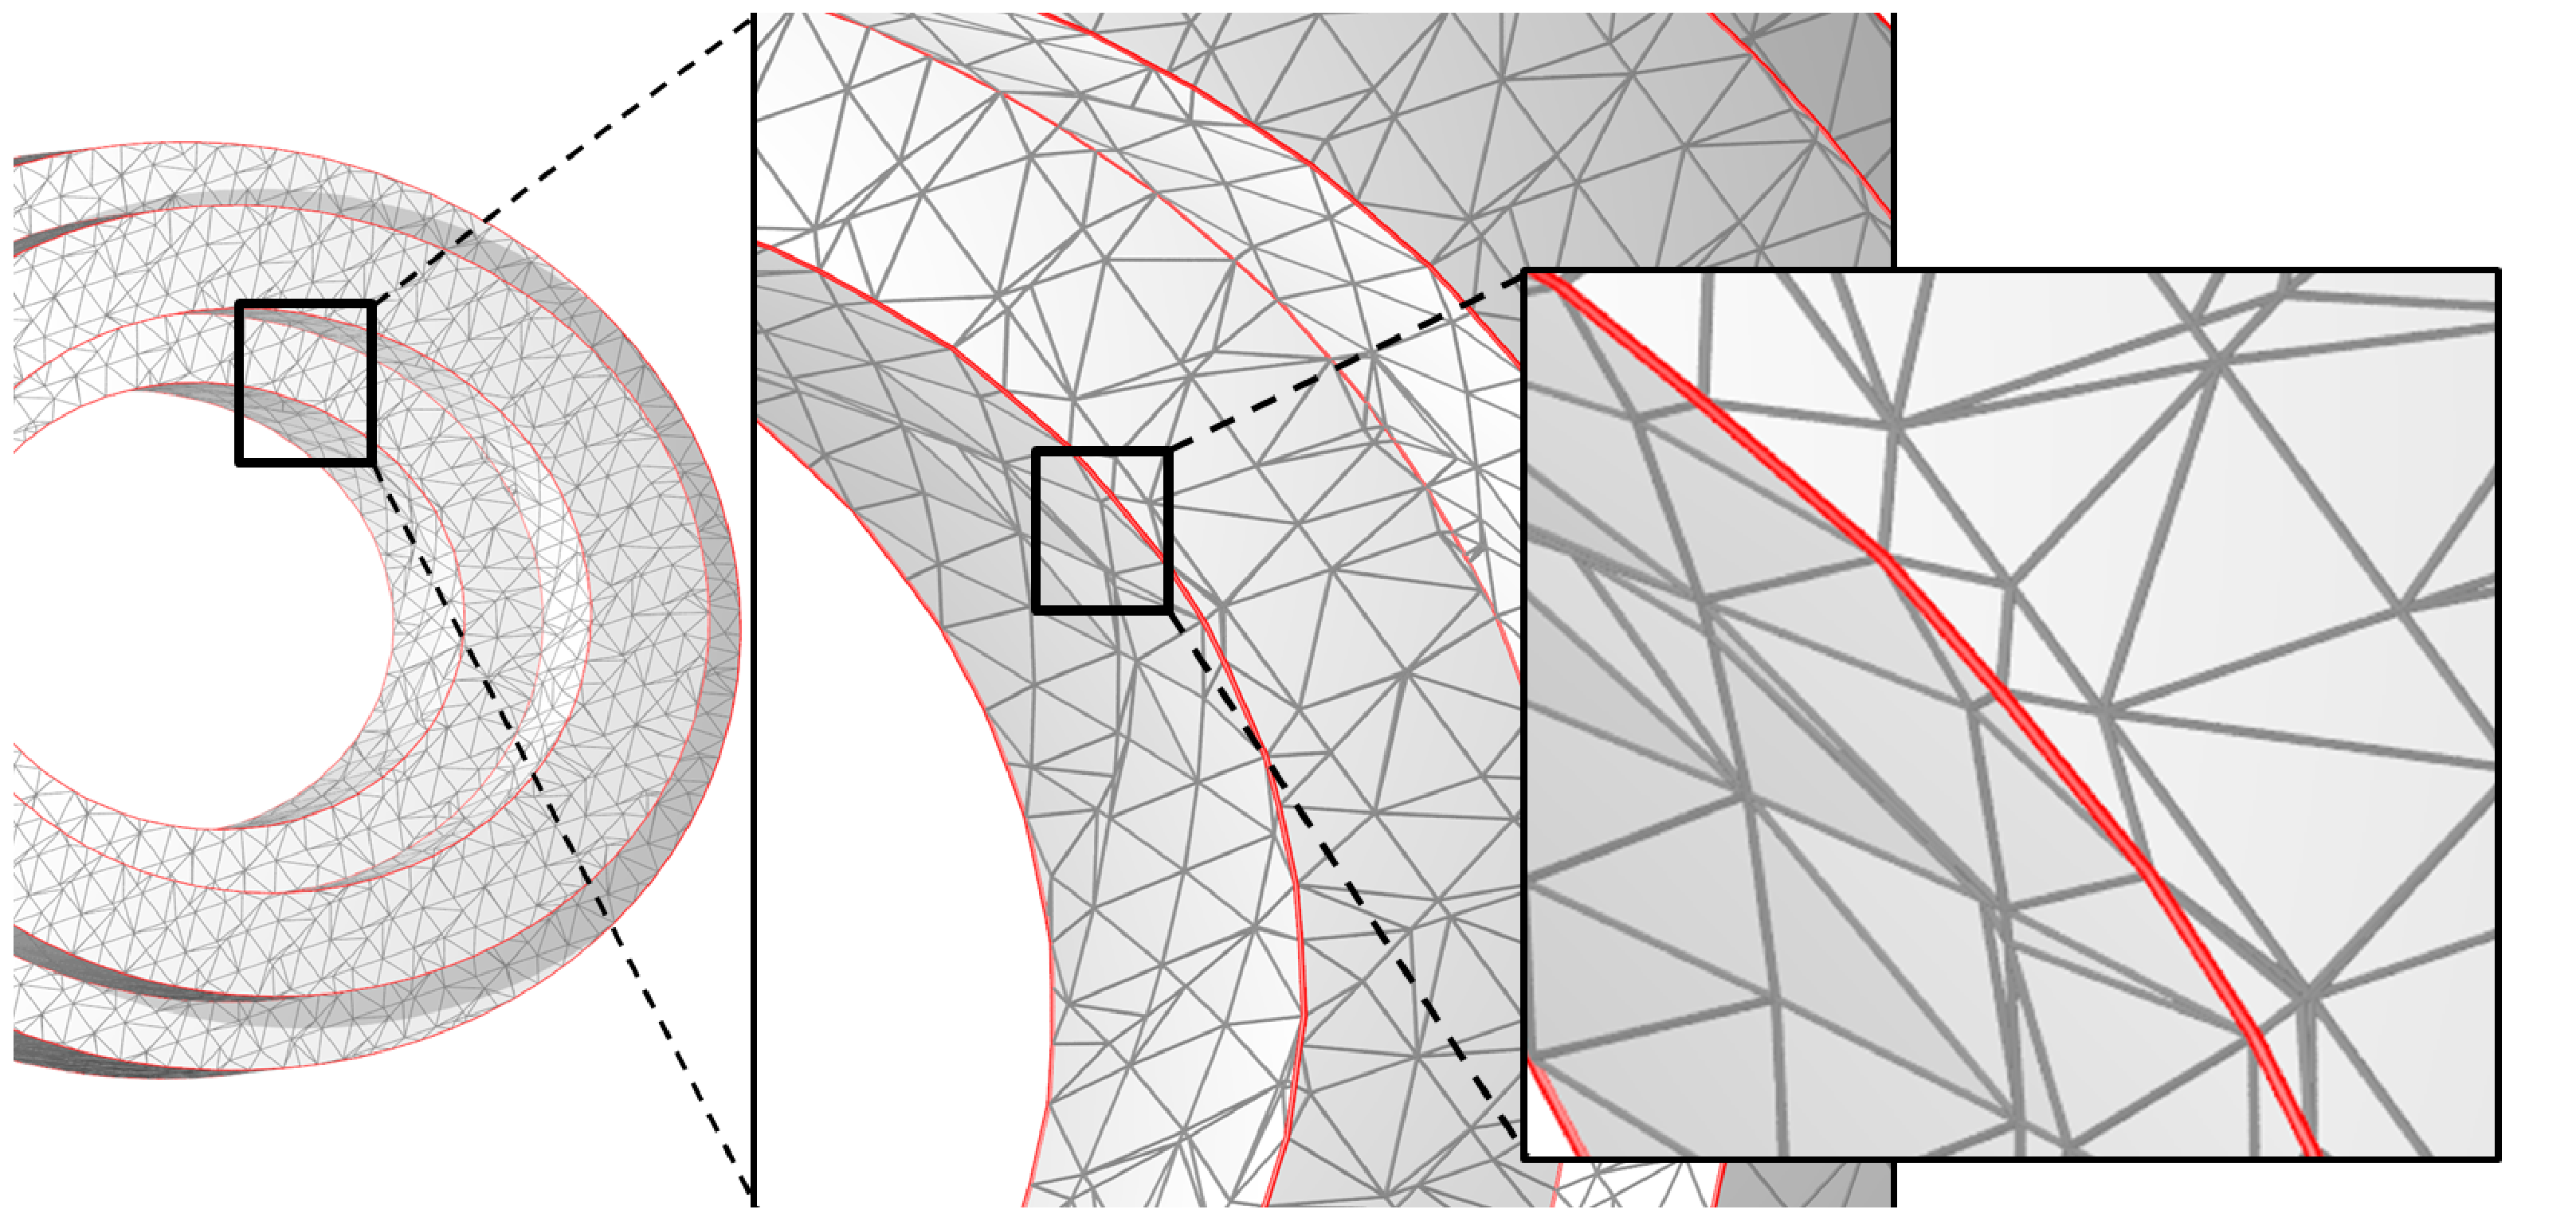
\includegraphics[width=0.5\linewidth]{images/isoExFlange.eps}\label{fig:isoEx:a} }
	\subfloat[]{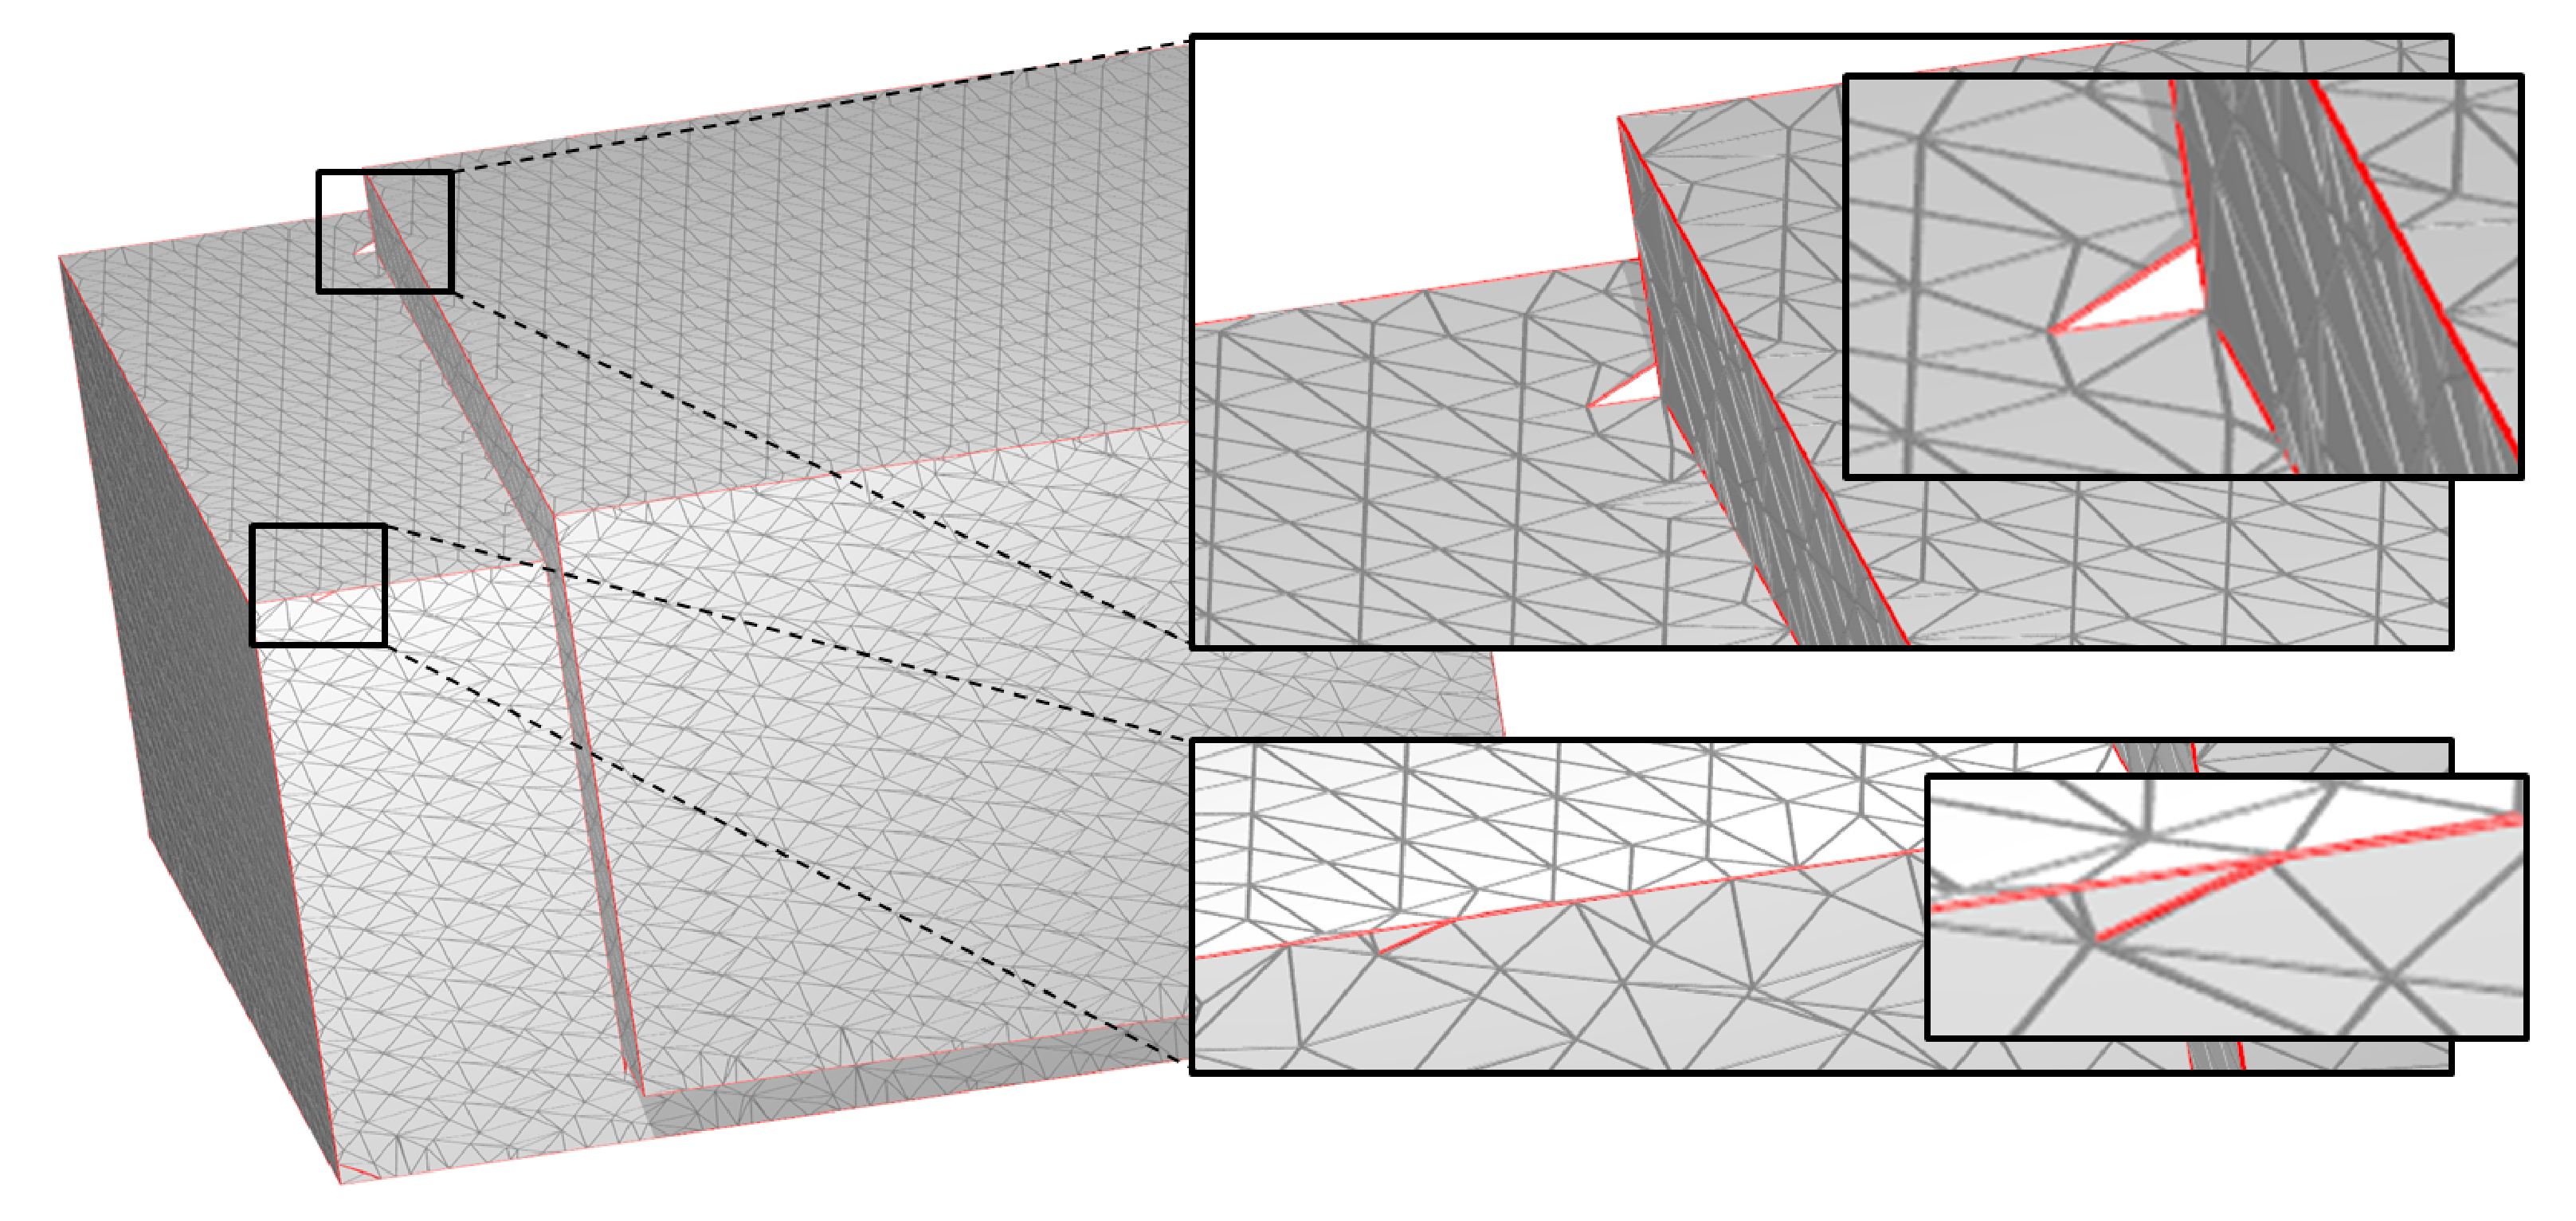
\includegraphics[width=0.5\linewidth]{images/isoExTwoCube.eps}\label{fig:isoEx:b}}
	\caption{Extended Marching Cubes results. (a) Extended Marching Cubes on a Flange dataset. (b) Extended Marching Cubes on a TwoCube dataset.}	
\end{figure}
We also compare our algorithm to Extended Marching Cubes by Kobbelt et al.~\cite{kbsh-fssev-01}. Figure~\protect\subref*{fig:isoEx:a},~\protect\subref*{fig:isoEx:b} shows the results of running Extended Marching Cubes on a Flange and a TwoCube dataset respectively. The magnified regions show that Extended Marching Cubes (same as Marching Cubes) is prone to producing small triangles. Occasionally Extended Marching Cubes also produces creases. 
\subsection{Timings}

